
% ////////////////////////////////////////////////

\begin{titlepage}
    \begin{figure}[H]
    \centering
    \begin{subfigure}{0.18\textwidth} 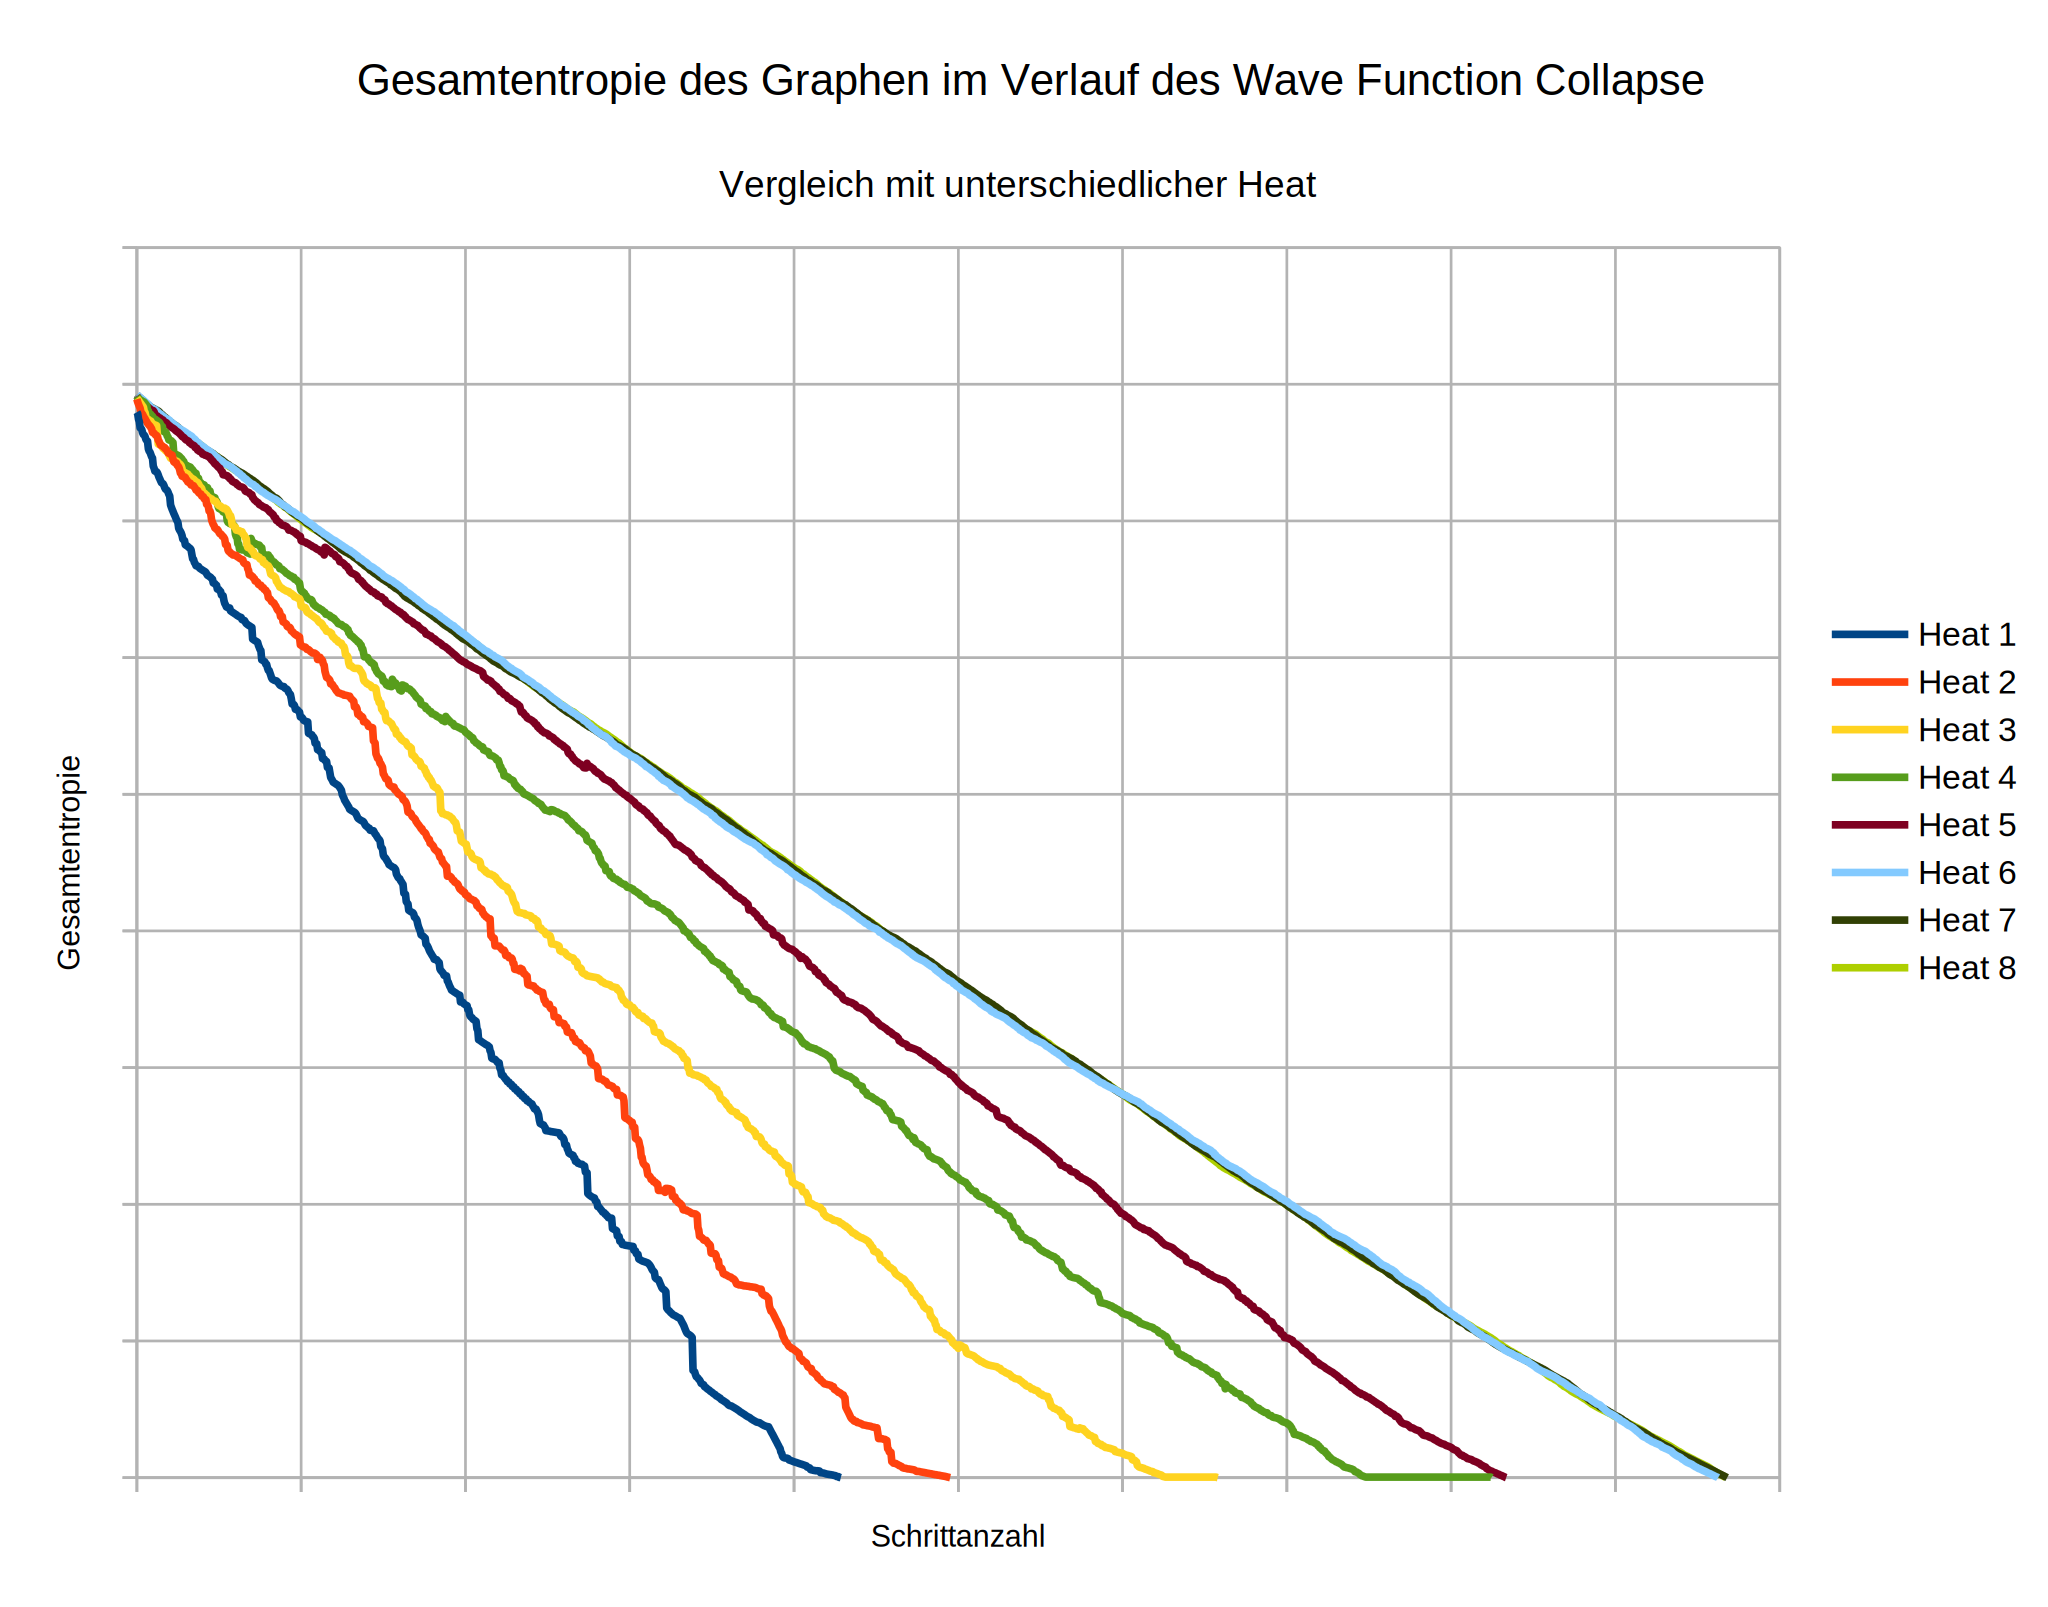
\includegraphics[width=\linewidth]{data/townscaper_grid/1.png} \caption{} \end{subfigure}
    \begin{subfigure}{0.18\textwidth} \includegraphics[width=\linewidth]{data/townscaper_grid/2.png} \caption{} \end{subfigure}
    \begin{subfigure}{0.18\textwidth} \includegraphics[width=\linewidth]{data/townscaper_grid/3.png} \caption{} \end{subfigure}
    \begin{subfigure}{0.18\textwidth} \includegraphics[width=\linewidth]{data/townscaper_grid/4.png} \caption{} \end{subfigure}
    \begin{subfigure}{0.18\textwidth} \includegraphics[width=\linewidth]{data/townscaper_grid/5.png} \caption{} \end{subfigure}
    
    \caption{
        Generierung eines Teils des Gitters für Townscaper \cite{stalberg_grid}. (a) Punkte werden generiert. (b) Triangulierung. (c) Kanten werden gelöscht, so dass Vierecke entstehen. (d) die Vierecke werden geviertelt. (e) Position der Knoten wird aufgelockert, so dass die Winkel zwischen Kanten gleichmäßiger sind.
    }
    \label{fig:townscaper_grid}
\end{figure}
    
    \begin{verbatim}
        
        
    \end{verbatim}
    
    \begin{center}
        \Large{Hochschule Anhalt}\\
        \Large{Fachbereich Informatik und Sprachen}\\
    \end{center}
    
    \begin{verbatim}
        
        
    \end{verbatim}
        
    \begin{center}
        \doublespacing
        \textbf{\LARGE{Bachelorarbeit}}\\
        \begin{verbatim}
            
        \end{verbatim}
        \textbf{\LARGE{Wave Function Collapse auf Graphen}}\\
        \singlespacing
        \begin{verbatim}
            
        \end{verbatim}
    \end{center}
    \begin{verbatim}
        
        
        
    \end{verbatim}
    \begin{flushleft}
        \begin{tabular}{llll}
            \textbf{Studiengang:} & & Angewandet Informatik: Digitale Medien und Spieleentwicklung & \\
            & & \\
            \textbf{Autor:} & & Name: Viktor Graf von Westarp & \\
            & & Matrikelnummer: 5058639 & \\
            & & E-Mail: viktor.grafvonwestarp@student.hs-anhalt.de & \\
            & & \\
            \textbf{Abgabedatum:} & & 5.\,Dezember\,2025 &\\
            & & \\
            \textbf{Betreuer:} & & Prof.\,Dr.\,Stefan Schlechtweg &\\
            \textbf{Zweitgutachterin:} & & Prof.\,Dr.\,Anika Groß &\\
        \end{tabular}
    \end{flushleft}
\end{titlepage}



% ////////////////////////////////////////////////

\tableofcontents

% ////////////////////////////////////////////////



\chapter*{Zusammenfassung}
\begin{quote}

Es wird eine Erweiterung des \textit{Wave Function Collapse} Algorithmus, die aus einem Beispiel ähnliche Ausgaben nicht nur wie zuvor auf regelmäßigen Gittern, sondern nun auch auf beliebigen Graphen, prozedural generieren kann, präsentiert. 
Die unterliegenden Struktur der Ausgabe wird von der Struktur des Beispiel entkoppelt und es können komplexere oder gar zuvor unmögliche, Ausgaben erstellt werden, ohne dass das Beispiel für diese angepasst werden muss. 
Ein neues Konzept namens \textit{Heat} definiert wie der Algorithmus die, aus dem Beispiel extrahierten, Regeln auf die Knoten des Graphen und deren Nachbarknoten anwendet. Dadurch können die Knoten beliebig angeordnet werden, anstatt auf ein Gitter beschränkt zu sein. Desweiteren wird Backtracking in der Generierung eingeführt, um die Laufzeit zu verbessern. Es wird auch gezeigt wie die, für die Ausgabe genutzten, Graphen automatisch erzeugt werden.
Der erweiterte Algorithmus kann mit dem selben Beispiel erfolgreich eine Vielzahl an Ausgaben auf unterschiedlichen Graphen generieren. Die Qualität der generierten Ausgabe hängt in gleichen Teilen von dem Beispiel, dem Graphen und der gewählten Heat ab. Diese Beziehung wird genauer untersucht.
Es wurde sich auf zweidimensionale Graphen beschränkt. Außerdem ist Heat als globaler, graphweiter Wert definiert. Dies macht die Methode besonders geeignet für Graphen mit relativ gleichmäßig verteilten Knoten. Bei stark unregelmäßige Graphstrukturen scheitert der Algorithmus häufiger oder kann nie eine zufriedenstellende Ausgabe generieren.

\end{quote}






\chapter{Einleitung}
    Diese Kapitel erklärt zuerst die Motivation hinter dieser Arbeit und geht auf das zulösende Problem und das genaue Ziel dieser Arbeit ein. Danach wird ein Überblick den Aufbau der Arbeit gegeben.
    
    \section{Motivation}
        Wave Function Collapse ist ein spannender Algorithmus, welcher, basiert auf einem einzigen Beispielmodell oder -bild, eine große Menge an ähnlichen Modellen und Bildern prozedural generieren kann. Bisher bestimmte die Form des Beispiels auch die Form des Ausgabe. Ein Beispielbild besteht aus Pixeln also werden auch Bilder aus Pixels generiert. Auch bei 3D Modellen beschränkt sich der Nutzer meist auf  z.B. würfelförmige Bauteile aus denen dann einen Modell zusammengestellt wird. Auch wenn der Innebereich solcher Bauteil beliebige Formen haben kann, werden die Bauteile dennoch würfelartig aneinander gebaut.
        
        Es muss aber nicht so sein, denn der Algorithmus selbst ist agnostisch gegenüber der Form der Ein- und Ausgabe. Es können nicht nur Bilder, sondern auch 3D Modelle generiert werden. Es sollte also möglich sein, dass der Algorithmus die Muster in einem Beispielbild auch auf eine anders geformte Struktur replizieren kann. Genauer sollten die Ausgabe nicht nur auf einem Gitter, sondern nun auch auf Graphen, geschehen können.
        
        Wäre dies möglich, so könnten Nutzer mit dem Algorithmus beliebige Strukturen als Basis nutzen und wären nicht mehr auf reine Gitter beschränkt. Dadurch könnten unregelmäßige oder organische Anordnungen, wie sind in der Natur, historischen Städten oder einem Mosaik vorkommen, als Basis für Ausgaben genutzt werden.
    
    
    
    \section{Problemstellung und Ziel}
        Ziel dieser Arbeit ist es, den Wave Function Collapse Algorithmus so erweitern, dass dieser eine Ausgabe auf Graphen generieren kann. Das heißt, dass die Struktur der Eingabe nicht mehr exakt zur Struktur der Ausgabe passen muss, sondern dass z.B. ein Beispielbild auf unterschiedlich strukturierte Graphen anwendbar sein soll, ohne dass das Beispielbild dafür verändert werden muss. 
        
        Das Kernproblem dabei ist, wie genau der Algorithmus die Informationen aus dem Beispielbild auf die Knoten eine Graphens einheitlich anwenden kann, wenn die Anordnung der Knoten und der Anzahl der Kanten pro Knoten im Graphen stark variieren können und keinerlei Ähnlichkeit zu dem Pixelgitter eines Bilds haben müssen. Gleichzeitig sollte der erweiterte Algorithmus immernoch die selbe Qualität für Ausgaben auf Gittern, als spezielle Art von Graphen, beibehalten. Insgesamt sollen die generierten Ausgaben eine gewisse Ähnlichkeit zum Beispiel haben, wobei diese vielleicht abgeschwächt werden muss. Dennoch sollte der Algorithmus eine hohe Ähnlichkeit erzielen.
    
    
    
    \section{Aufbau der Arbeit}
        Es folgen fünf Kapitel in dieser Arbeit. Zuerst werden grundlegende Begriffe erklärt und es wird ein Überblick über den Stand der Technik im Bereich Wave Function Collapse gegeben. Danach wird die Beschränkung des Algorithmus genauer beschrieben und darauf eingegangen wie der Algorithmus erweitert wird und welchen Änderungen es dafür bedarf. Danach wird erklärt wie diese Änderungen umgesetzt wurden. Es folgt ein Überblick über die erzielten Resultate und es wird genauer auf Aspekte der Erweiterung eingegangen. Schließlich folgt eine Zusammenfassung der Arbeit, in der auch auf die Vor- und die Nachteile genannt werden.




\chapter{Hintergrund}
    In diesem Kapitel werden zuerst einige grundlegende Begriffe erklärt. Danach wird auf die Algorithmen, auf denen diese Arbeit basiert, eingegangen. Dies sind \textit{Model Synthesis} von Merrel \cite{merrel} und dessen Weiterentwicklung \textit{Wave Function Collapse} von Gumin \cite{gumin}.
    
    \section{Begriffserklärung}
        Ein \textit{Gitter} beschreibt eine regelmäßig aufgebaute Struktur aus einzelnen Punkten. Diese Knotenpunkte sind durch Kanten mit ihren direkten Nachbarn verbunden. Ein Bild wird digital z.B. auf einem Gitter von Pixeln gespeichert und dargestellt. Genauso bilden die Kästchen eines Sudoku ein Gitter. Wenn solch ein Gitter in einer Ebene liegt, wird es auch als \textit{2D Gitter} bezeichnet. Sind die Punkte regelmäßig im Raum angeordnet spricht man von einem \textit{3D Gitter}. Ein \textit{Graph} besteht aus einer Menge an Knoten $V$ und einer Menge an Kanten $E$, wobei eine Kante ein Knotenpaar aus $V$ ($\{v_1, v_2\} \in V$) ist. Die Knotenpunkte können eine beliebige Anordnung haben und beliebig mit anderen Knoten durch Kanten verbunden sein. Ein Gitter ist eine spezielle Form eines Graphen, bei die Knoten enlang von festen Achsen angeordnet werden und nur Kanten entlang dieser Achse so den nächstliegenden Knoten existieren.
        \\
        \\
        Eine \textit{Triangulierung} ist ein Graph, dessen Knoten und Kanten Dreiecke aufspannen. Eine besonders wichtige Variante ist die \textit{Delaunay-Triangulierung} \cite{delaunay}, bei der die Dreiecke so gewählt werden, dass der kleinste Winkel innerhalb jedes Dreiecks möglichst groß ist. Dadurch entstehen „gut geformte“ Dreiecke. Eng verwandt damit ist das \textit{Voronoi-Diagramm} \cite{voronoi}. Es teilt die Ebene in Regionen auf, sodass jeder Punkt genau die Fläche erhält, die ihm am nächsten liegt. Die Delaunay-Triangulierung und das Voronoi-Diagramm sind dual zueinander: Verbindet man die Mittelpunkte der Voronoi-Zellen, entsteht die Delaunay-Triangulierung, und aus einer Delaunay-Triangulierung lässt sich wiederum das zugehörige Voronoi-Diagramm ableiten. In Abbildung \ref{fig:delaunay_voronoi} ist die Delaunay-Triangulierung und das Voronoi-Diagram für einige Punkte dargestellt.
        
        \begin{figure}[H]
    \centering
    \begin{subfigure}{0.18\textwidth} 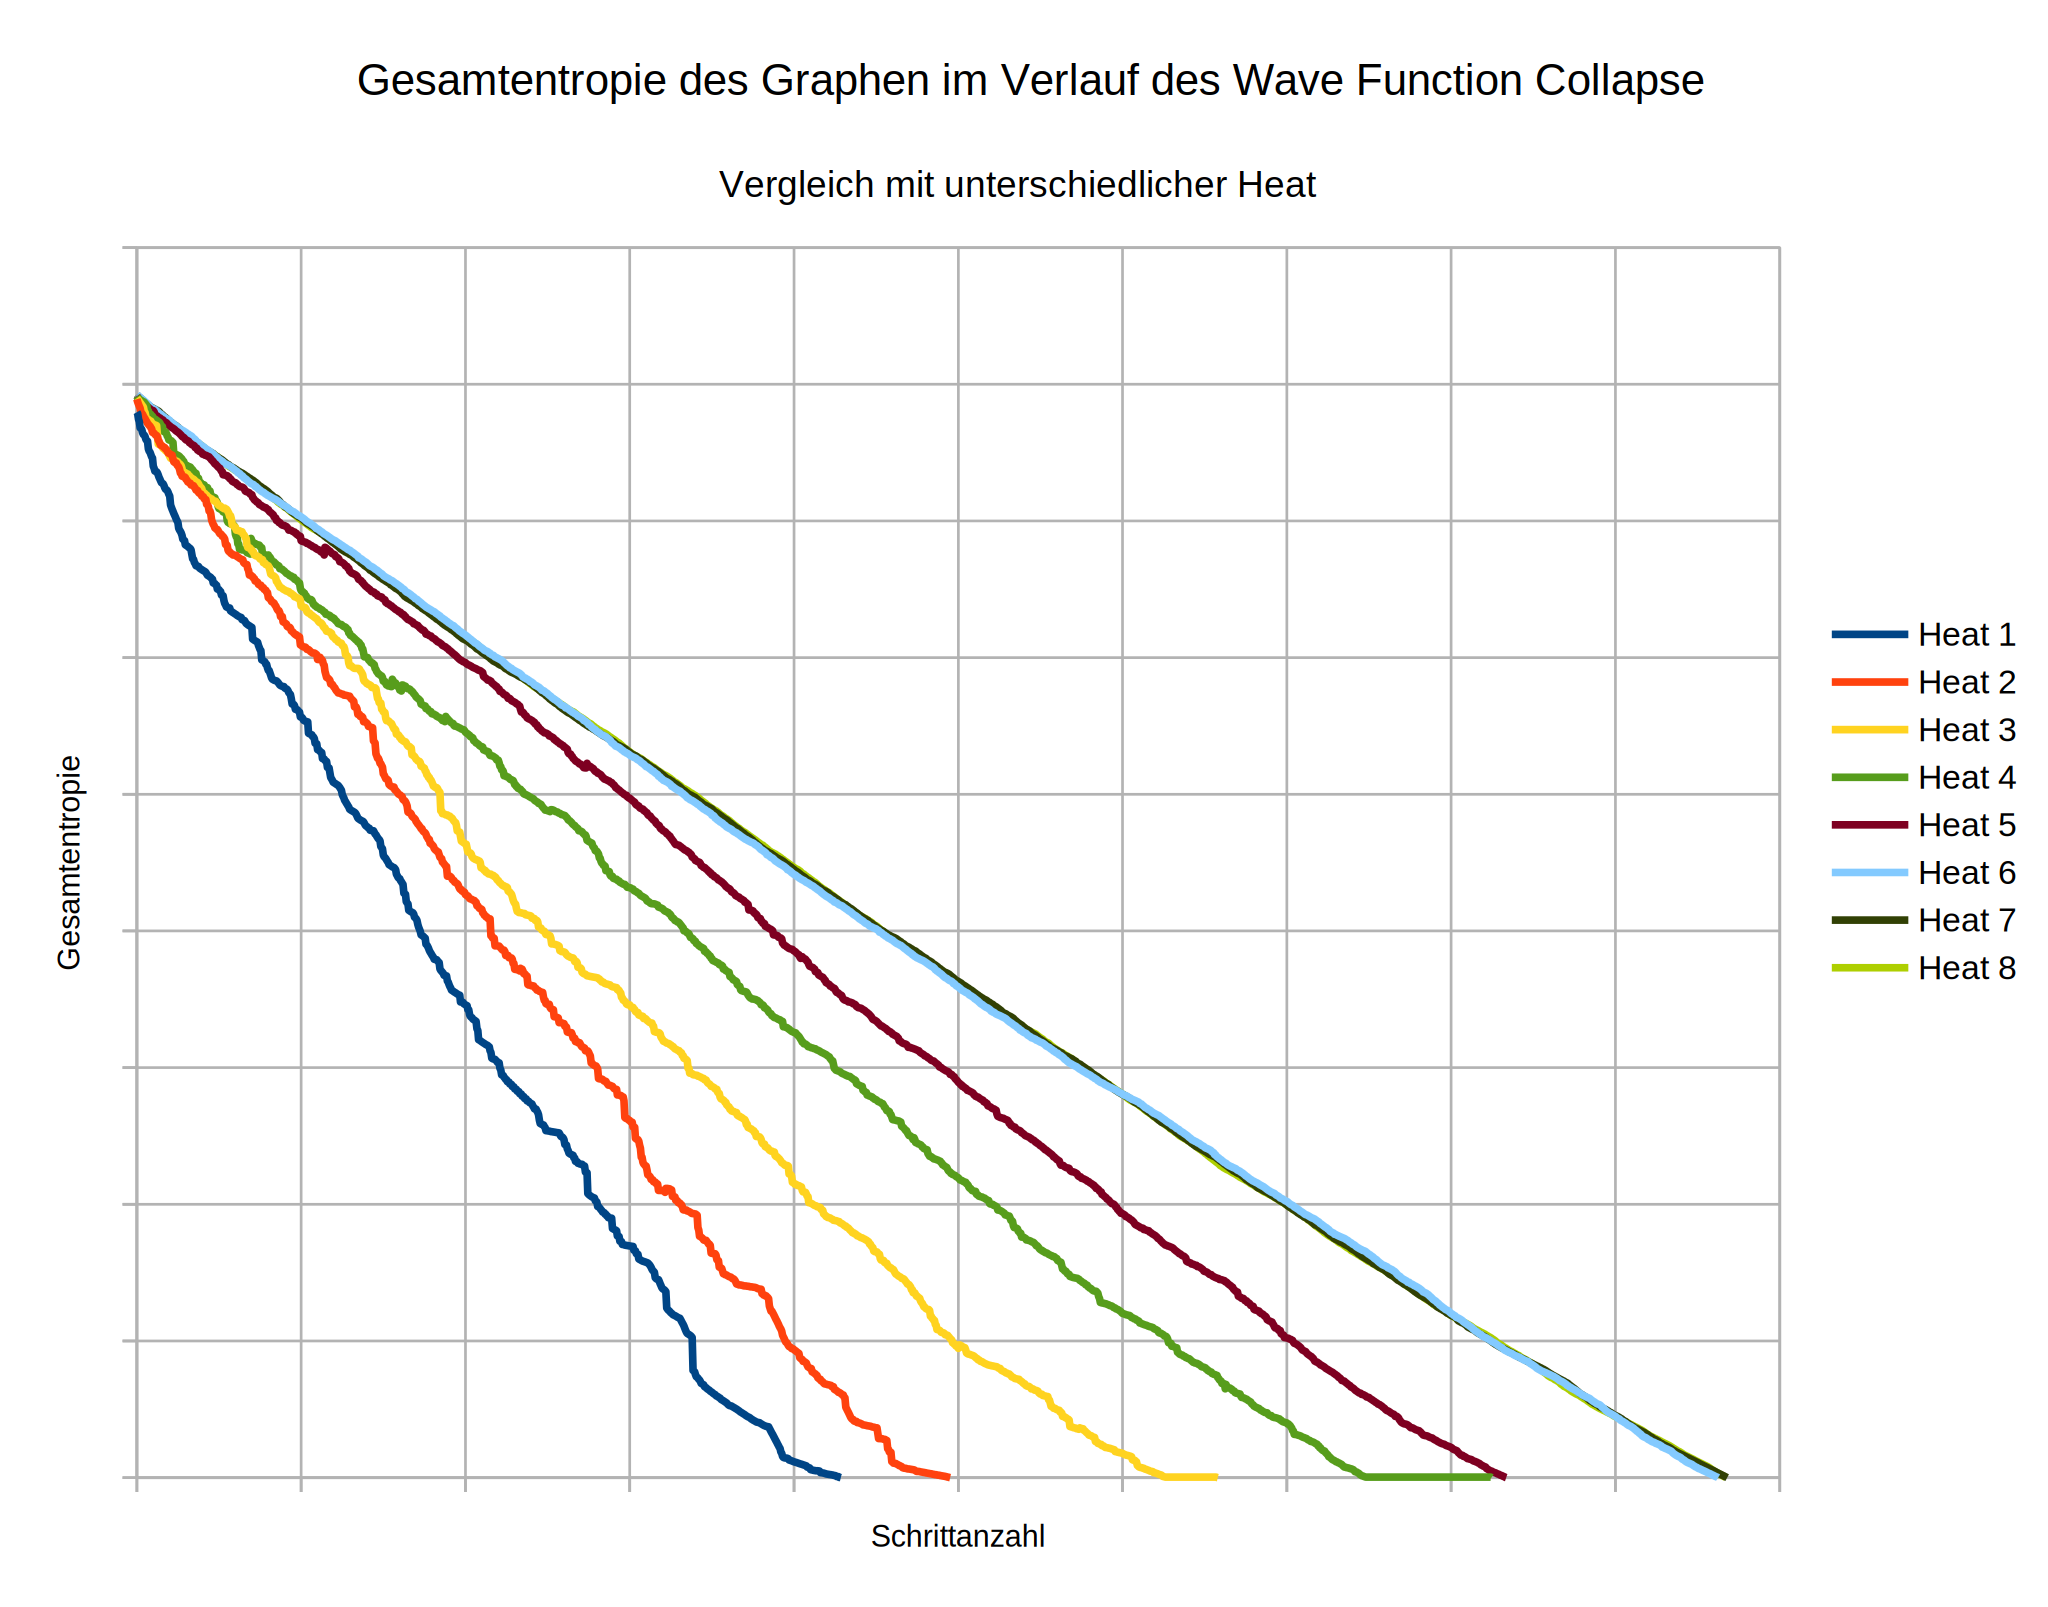
\includegraphics[width=\linewidth]{data/townscaper_grid/1.png} \caption{} \end{subfigure}
    \begin{subfigure}{0.18\textwidth} \includegraphics[width=\linewidth]{data/townscaper_grid/2.png} \caption{} \end{subfigure}
    \begin{subfigure}{0.18\textwidth} \includegraphics[width=\linewidth]{data/townscaper_grid/3.png} \caption{} \end{subfigure}
    \begin{subfigure}{0.18\textwidth} \includegraphics[width=\linewidth]{data/townscaper_grid/4.png} \caption{} \end{subfigure}
    \begin{subfigure}{0.18\textwidth} \includegraphics[width=\linewidth]{data/townscaper_grid/5.png} \caption{} \end{subfigure}
    
    \caption{
        Generierung eines Teils des Gitters für Townscaper \cite{stalberg_grid}. (a) Punkte werden generiert. (b) Triangulierung. (c) Kanten werden gelöscht, so dass Vierecke entstehen. (d) die Vierecke werden geviertelt. (e) Position der Knoten wird aufgelockert, so dass die Winkel zwischen Kanten gleichmäßiger sind.
    }
    \label{fig:townscaper_grid}
\end{figure}
        
        Unter \textit{Prozedurale Generierung} versteht man Algorithmen, die Inhalte wie z.B. Bilder, 3D Modelle oder Musik erzeugen können. Meist nimmt ein solcher Algorithmus nur eine kleine Menge an Daten als Eingabe und generiert daraus viele Variationen an Ausgaben. Dabei werden häufig Zufallszahl-Generatoren benutzt, aber der Ablauf ist nicht rein zufällig. Bei gleicher Initialisierung generiert ein solcher Algorithmus immer die selbe Ausgabe und kann durch Parameter gesteuert werden. Prozedurale Generierung wird in Computerspielen regelmäßig verwendet, da es den Entwicklern erlaubt den Spielern viele varierte Inhalte zu bieten, ohne diese alle vorher manuell anzufertigen und fest im Spiel einzubauen.
    
    \section{Model Synthesis}
        Mit dem \textit{Model Synthesis} \cite{merrel} Algorithmus \ref{alg:ms_merrel} können, basiert auf einem 3D Beispielmodell, eine große Menge an ähnlichen 3D Modellen prozedural generiert werden (siehe Abbildung \ref{fig:ms_output}). Das Beispielmodell muss zuvor in kleinere Bauteile zerlegt werden, aus denen der Algorithmus dann ein neues Modell generiert. Ein Bauteil kann ein komplexer Teil des Beispiels sein, kann aber auch einen leeren Teil des Beispiels enthalten. Die Bauteile werden wie Bauklötze zusammengebaut, wobei zwei Bauteile nur dann nebeneinander platziert werden dürfen, wenn diese auch im Beispielmodell nebeneinander vorkommen. Diese Eigenschaft wird auch Konsistenz genannt. Ein simples konsistentes Modell ist z.B. ein leeres Modell.
        
        Der Algorithmus arbeitet auf einem 3D Gitter. Jedem Knotenpunkt des Gitters wird im fertigen Modell ein Bauteil zugewiesen, doch vorher könnten an jedem Knotenpunkt mehrere Bauteile ein konsistentes Modell bilden. Der Algorithmus wählt iterativ ein Bauteil und prüft, dass dadurch kein anderer Knotenpunkt nun keine möglichen Bauteile mehr hat. Wäre dies der Fall, so könnte das Modell nicht mehr vervollständigt werden. Hierfür wird eine globale Suche verwendet, andere Methoden beschränkten sich zuvor nur auf lokale Suchen. Eine globale Suche hat zum Vorteil, dass auch ein weitreichenden Einfluss eines Bauteils auf das gesamte Gitter korrekt behandelt wird. Die Auswahl der Bauteile geschieht per Zufall, dabei werden Bauteile die oft im Beispiel vorkommen wahrscheinlicher ausgewählt als seltene Bauteile. Für eine generiertes Modell bedeutet dies, dass die globale Verteilung der Bauteile auch tendenziell der Verteilung im Beispiel gleicht.
        
        \begin{figure}[H]
    \centering
    \begin{subfigure}{0.18\textwidth} 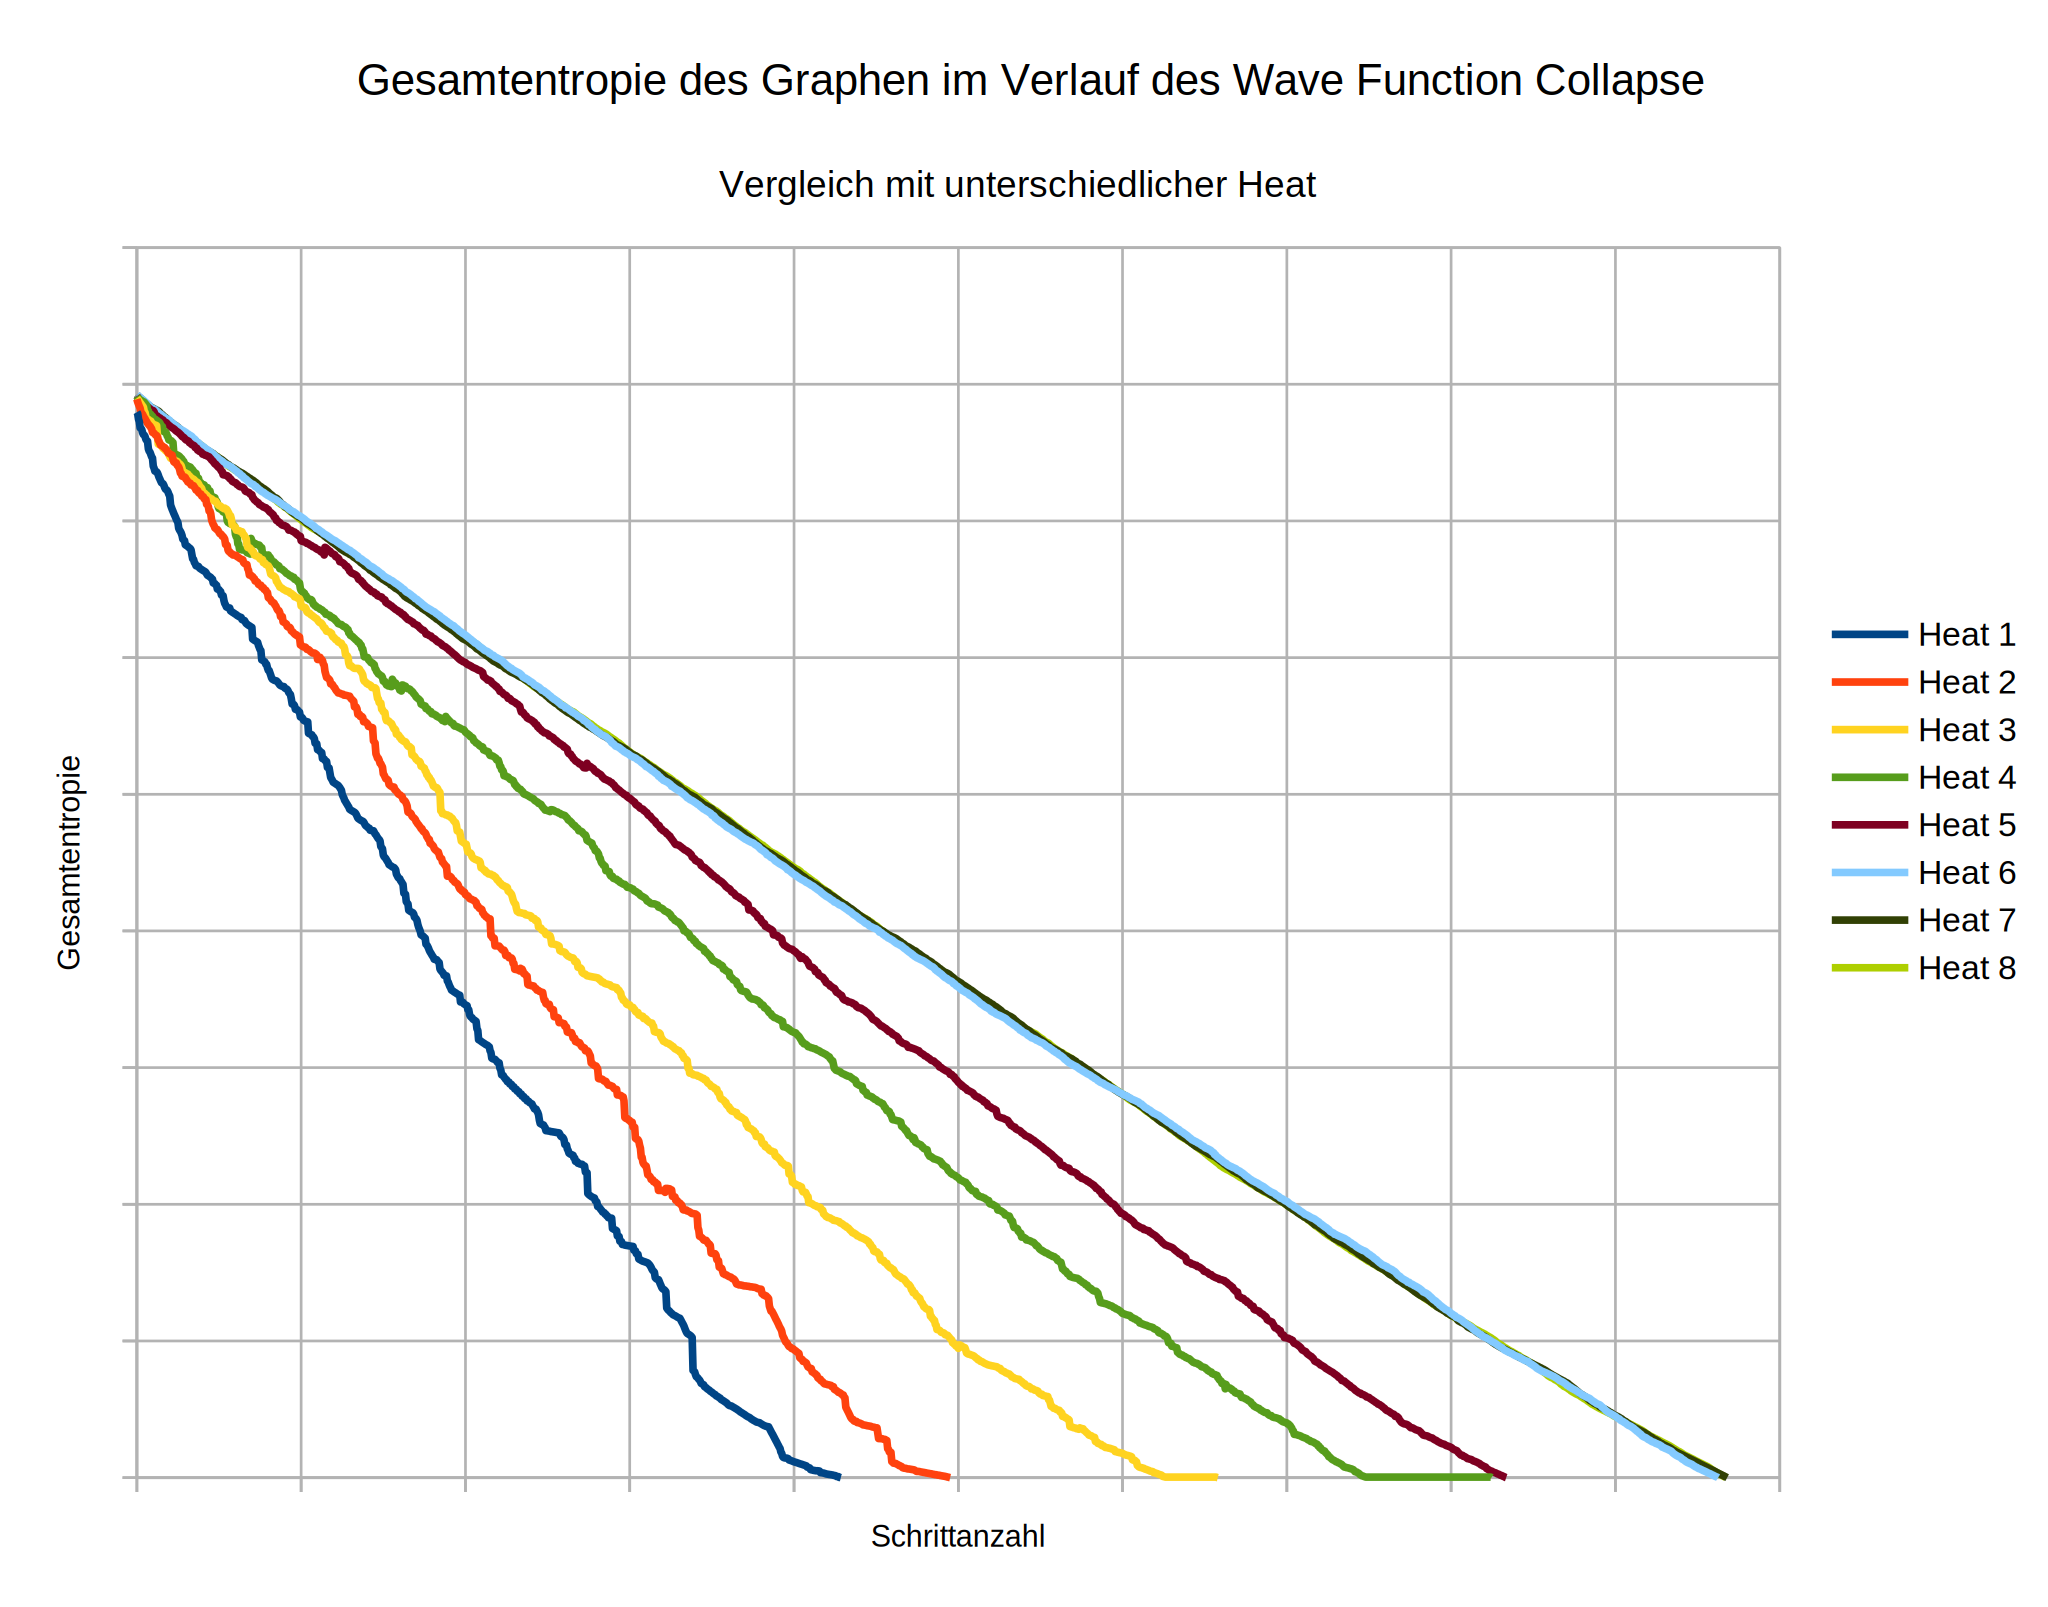
\includegraphics[width=\linewidth]{data/townscaper_grid/1.png} \caption{} \end{subfigure}
    \begin{subfigure}{0.18\textwidth} \includegraphics[width=\linewidth]{data/townscaper_grid/2.png} \caption{} \end{subfigure}
    \begin{subfigure}{0.18\textwidth} \includegraphics[width=\linewidth]{data/townscaper_grid/3.png} \caption{} \end{subfigure}
    \begin{subfigure}{0.18\textwidth} \includegraphics[width=\linewidth]{data/townscaper_grid/4.png} \caption{} \end{subfigure}
    \begin{subfigure}{0.18\textwidth} \includegraphics[width=\linewidth]{data/townscaper_grid/5.png} \caption{} \end{subfigure}
    
    \caption{
        Generierung eines Teils des Gitters für Townscaper \cite{stalberg_grid}. (a) Punkte werden generiert. (b) Triangulierung. (c) Kanten werden gelöscht, so dass Vierecke entstehen. (d) die Vierecke werden geviertelt. (e) Position der Knoten wird aufgelockert, so dass die Winkel zwischen Kanten gleichmäßiger sind.
    }
    \label{fig:townscaper_grid}
\end{figure}
        \begin{figure}[H]
    \centering
    \begin{minipage}{\linewidth}
        \rule{\linewidth}{0.4pt}
         
        \begin{enumerate}
        \item $M_0$ ist ein simples konsitentes Modell. $M = M_0$
        \subitem Wiederhole 2. bis 5. bis jeder Teil des Modells angepasst wurde
        \item Wähle eine Menge $B$ an Knotenpunkten zur Bearbeitung
        \item  $M' = M$ ohne die Knotenpunkte $B$ und deren bisherigen Bauteilen
        \item Arbeite alle Knotenpunkte von $B$ ab:
        \subitem Wähle einen Knotenpunkte aus und weise ihm ein konsistentes Bauteil zu
        \subitem Ist $M'$ nicht mehr konsistent, dann brich ab
        \subitem Füge diesen Knotenpunkt in $M'$ ein
        \item Wenn $M'$ noch konsistent ist, dann $M = M'$
        \end{enumerate}
        
        \rule{\linewidth}{0.4pt}
    \end{minipage}
    
    \caption{Model Synthesis Algorithmus nach Merrel \cite{merrel}}
    
    \label{fig:ms_merrel}
\end{figure}
        \begin{figure}[H]
    \centering
    \begin{subfigure}{0.18\textwidth} 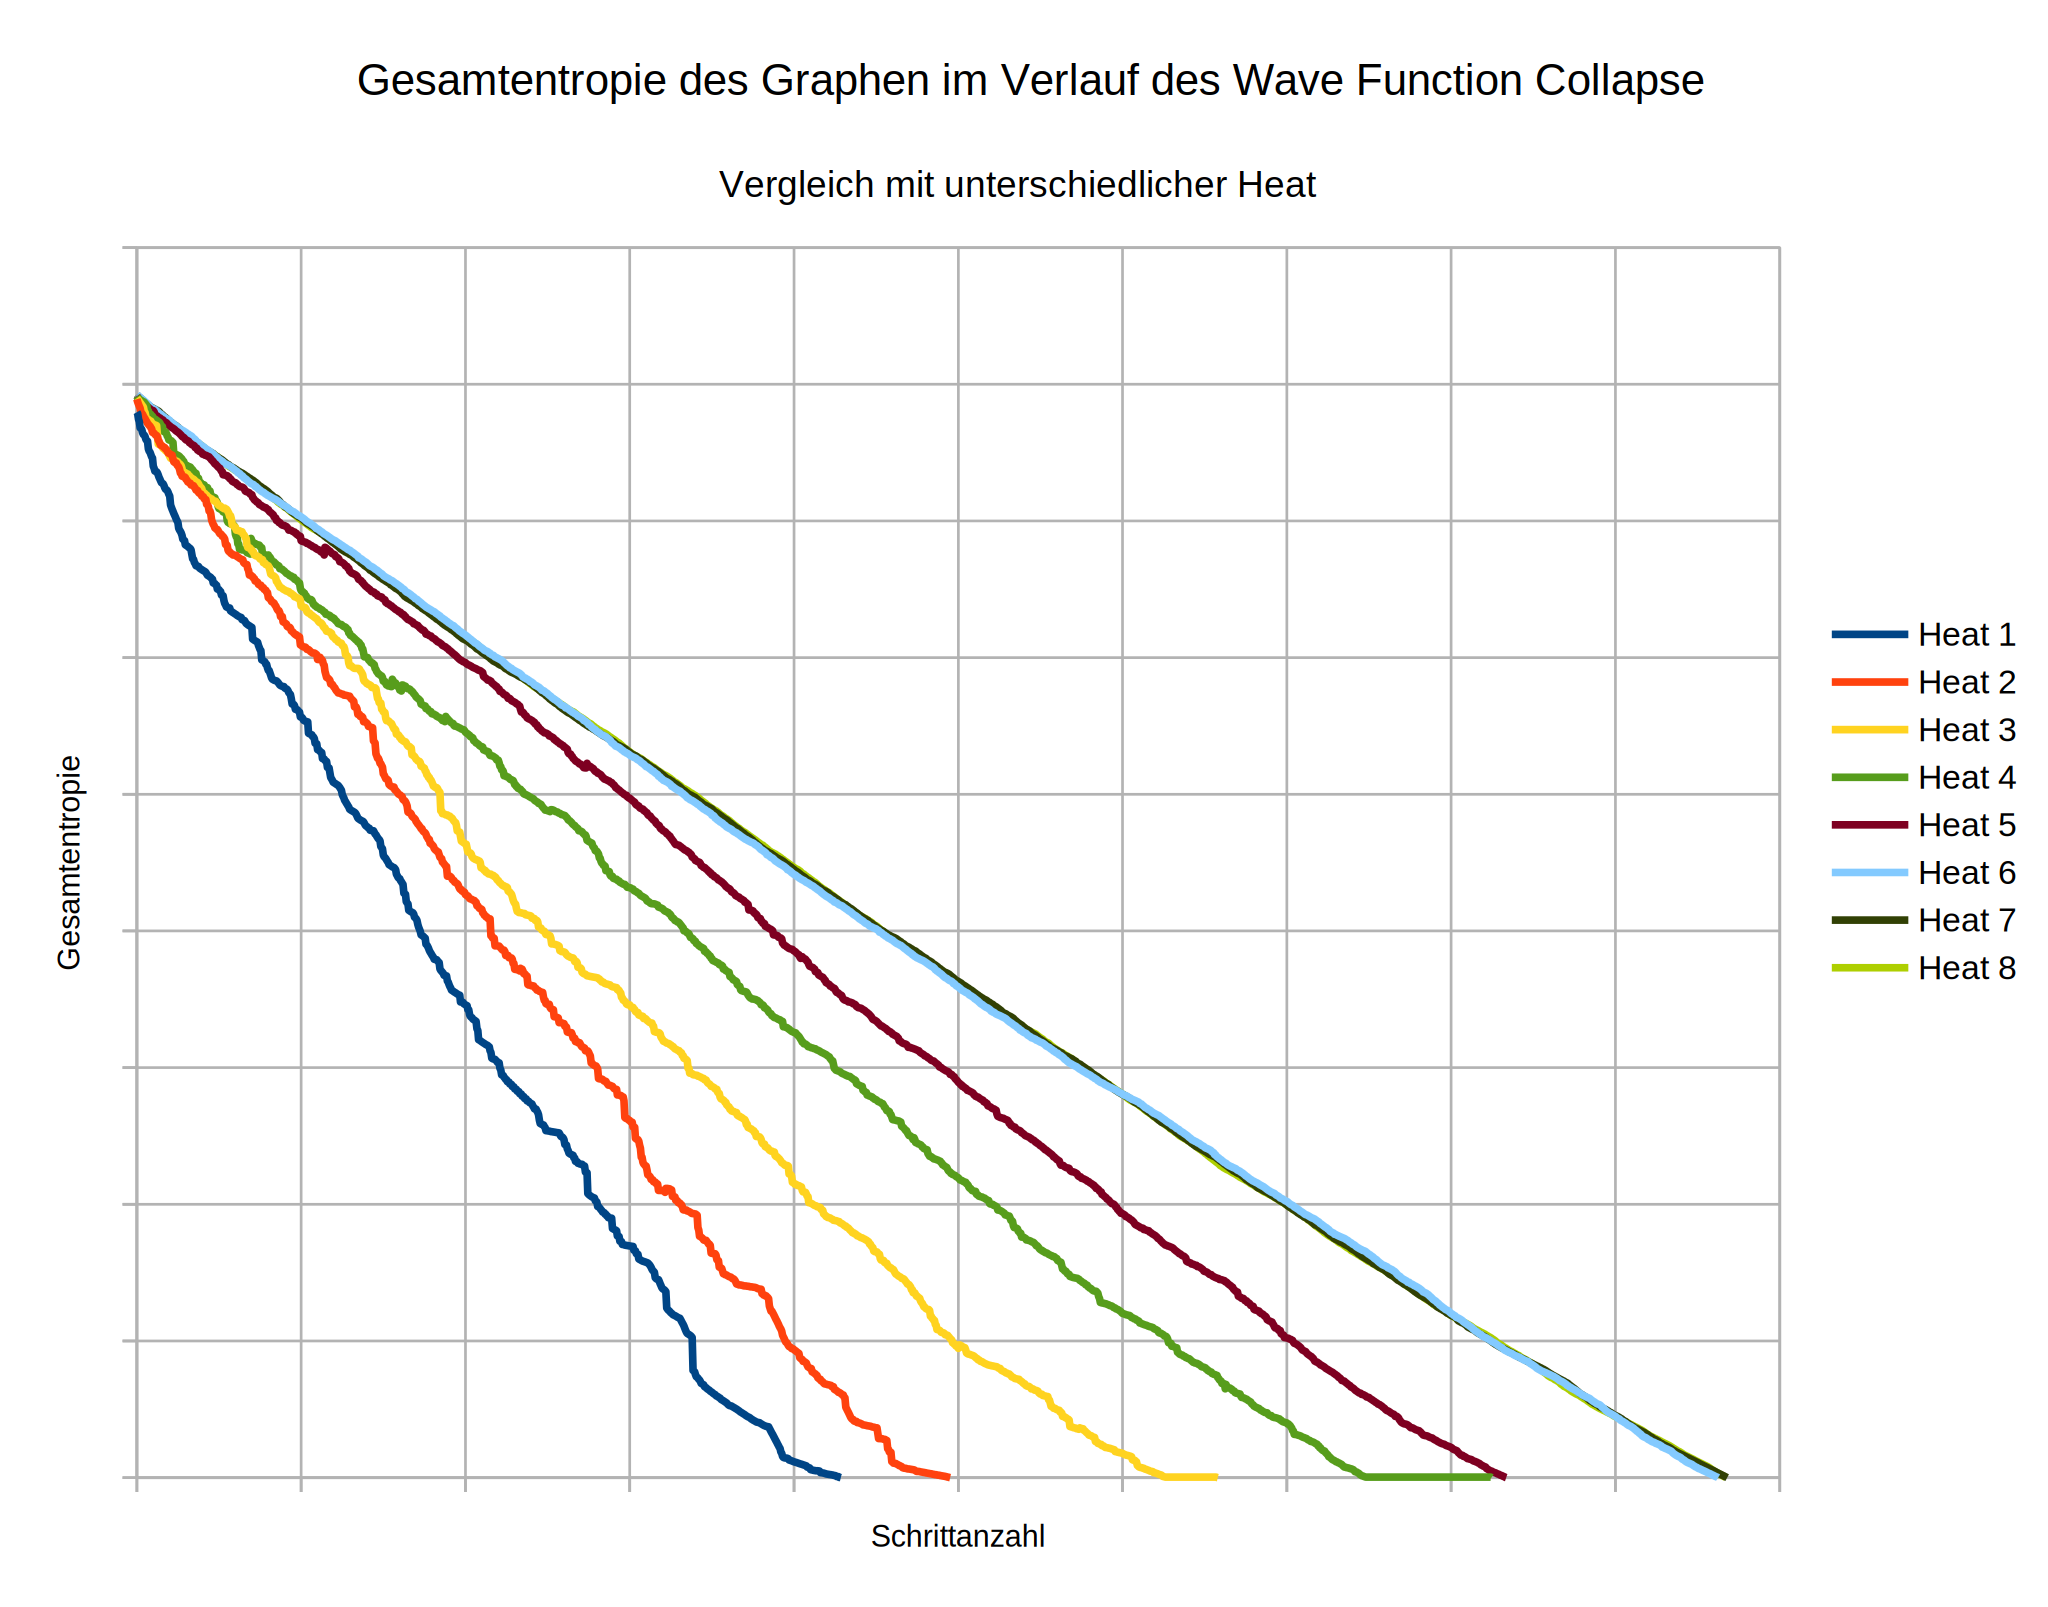
\includegraphics[width=\linewidth]{data/townscaper_grid/1.png} \caption{} \end{subfigure}
    \begin{subfigure}{0.18\textwidth} \includegraphics[width=\linewidth]{data/townscaper_grid/2.png} \caption{} \end{subfigure}
    \begin{subfigure}{0.18\textwidth} \includegraphics[width=\linewidth]{data/townscaper_grid/3.png} \caption{} \end{subfigure}
    \begin{subfigure}{0.18\textwidth} \includegraphics[width=\linewidth]{data/townscaper_grid/4.png} \caption{} \end{subfigure}
    \begin{subfigure}{0.18\textwidth} \includegraphics[width=\linewidth]{data/townscaper_grid/5.png} \caption{} \end{subfigure}
    
    \caption{
        Generierung eines Teils des Gitters für Townscaper \cite{stalberg_grid}. (a) Punkte werden generiert. (b) Triangulierung. (c) Kanten werden gelöscht, so dass Vierecke entstehen. (d) die Vierecke werden geviertelt. (e) Position der Knoten wird aufgelockert, so dass die Winkel zwischen Kanten gleichmäßiger sind.
    }
    \label{fig:townscaper_grid}
\end{figure}
        
        Die selbe Methodik kann auch für Beispielbilder benutzt werden, dies wird dann auch \textit{Texture Synthesis} genannt. In diesem Fall arbeitet der Algorithmus mit 2D Gittern und Bauteilen. Die Ausgabe des Algorithmus kann auch durch Soft-Constraints beschränkt werden (siehe Abbildung \ref{fig:ms_constrained}). Ebenso kann Symmetrie, Spiegelung und Drehung, in der Ausgabe erzwungen werden. Beide Ansätze wurden nicht weiter in dieser Arbeit betrachetet. Es wird empfohlen, dass der Algorithmus nicht das ganze Gitter auf einmal löst, damit Widersprüche nicht zu einem kompletten Neustart führen. Stattdessen sollen iterativ kleine Abschnitte für sich solange gelöst werden bis eine valide Ausgabe entsteht (siehe Abbildung \ref{fig:ms_algorithm}). In dieser Arbeit wurde darauf verzichtet.
        
        \begin{figure}[H]
    \centering
    \begin{subfigure}{0.18\textwidth} 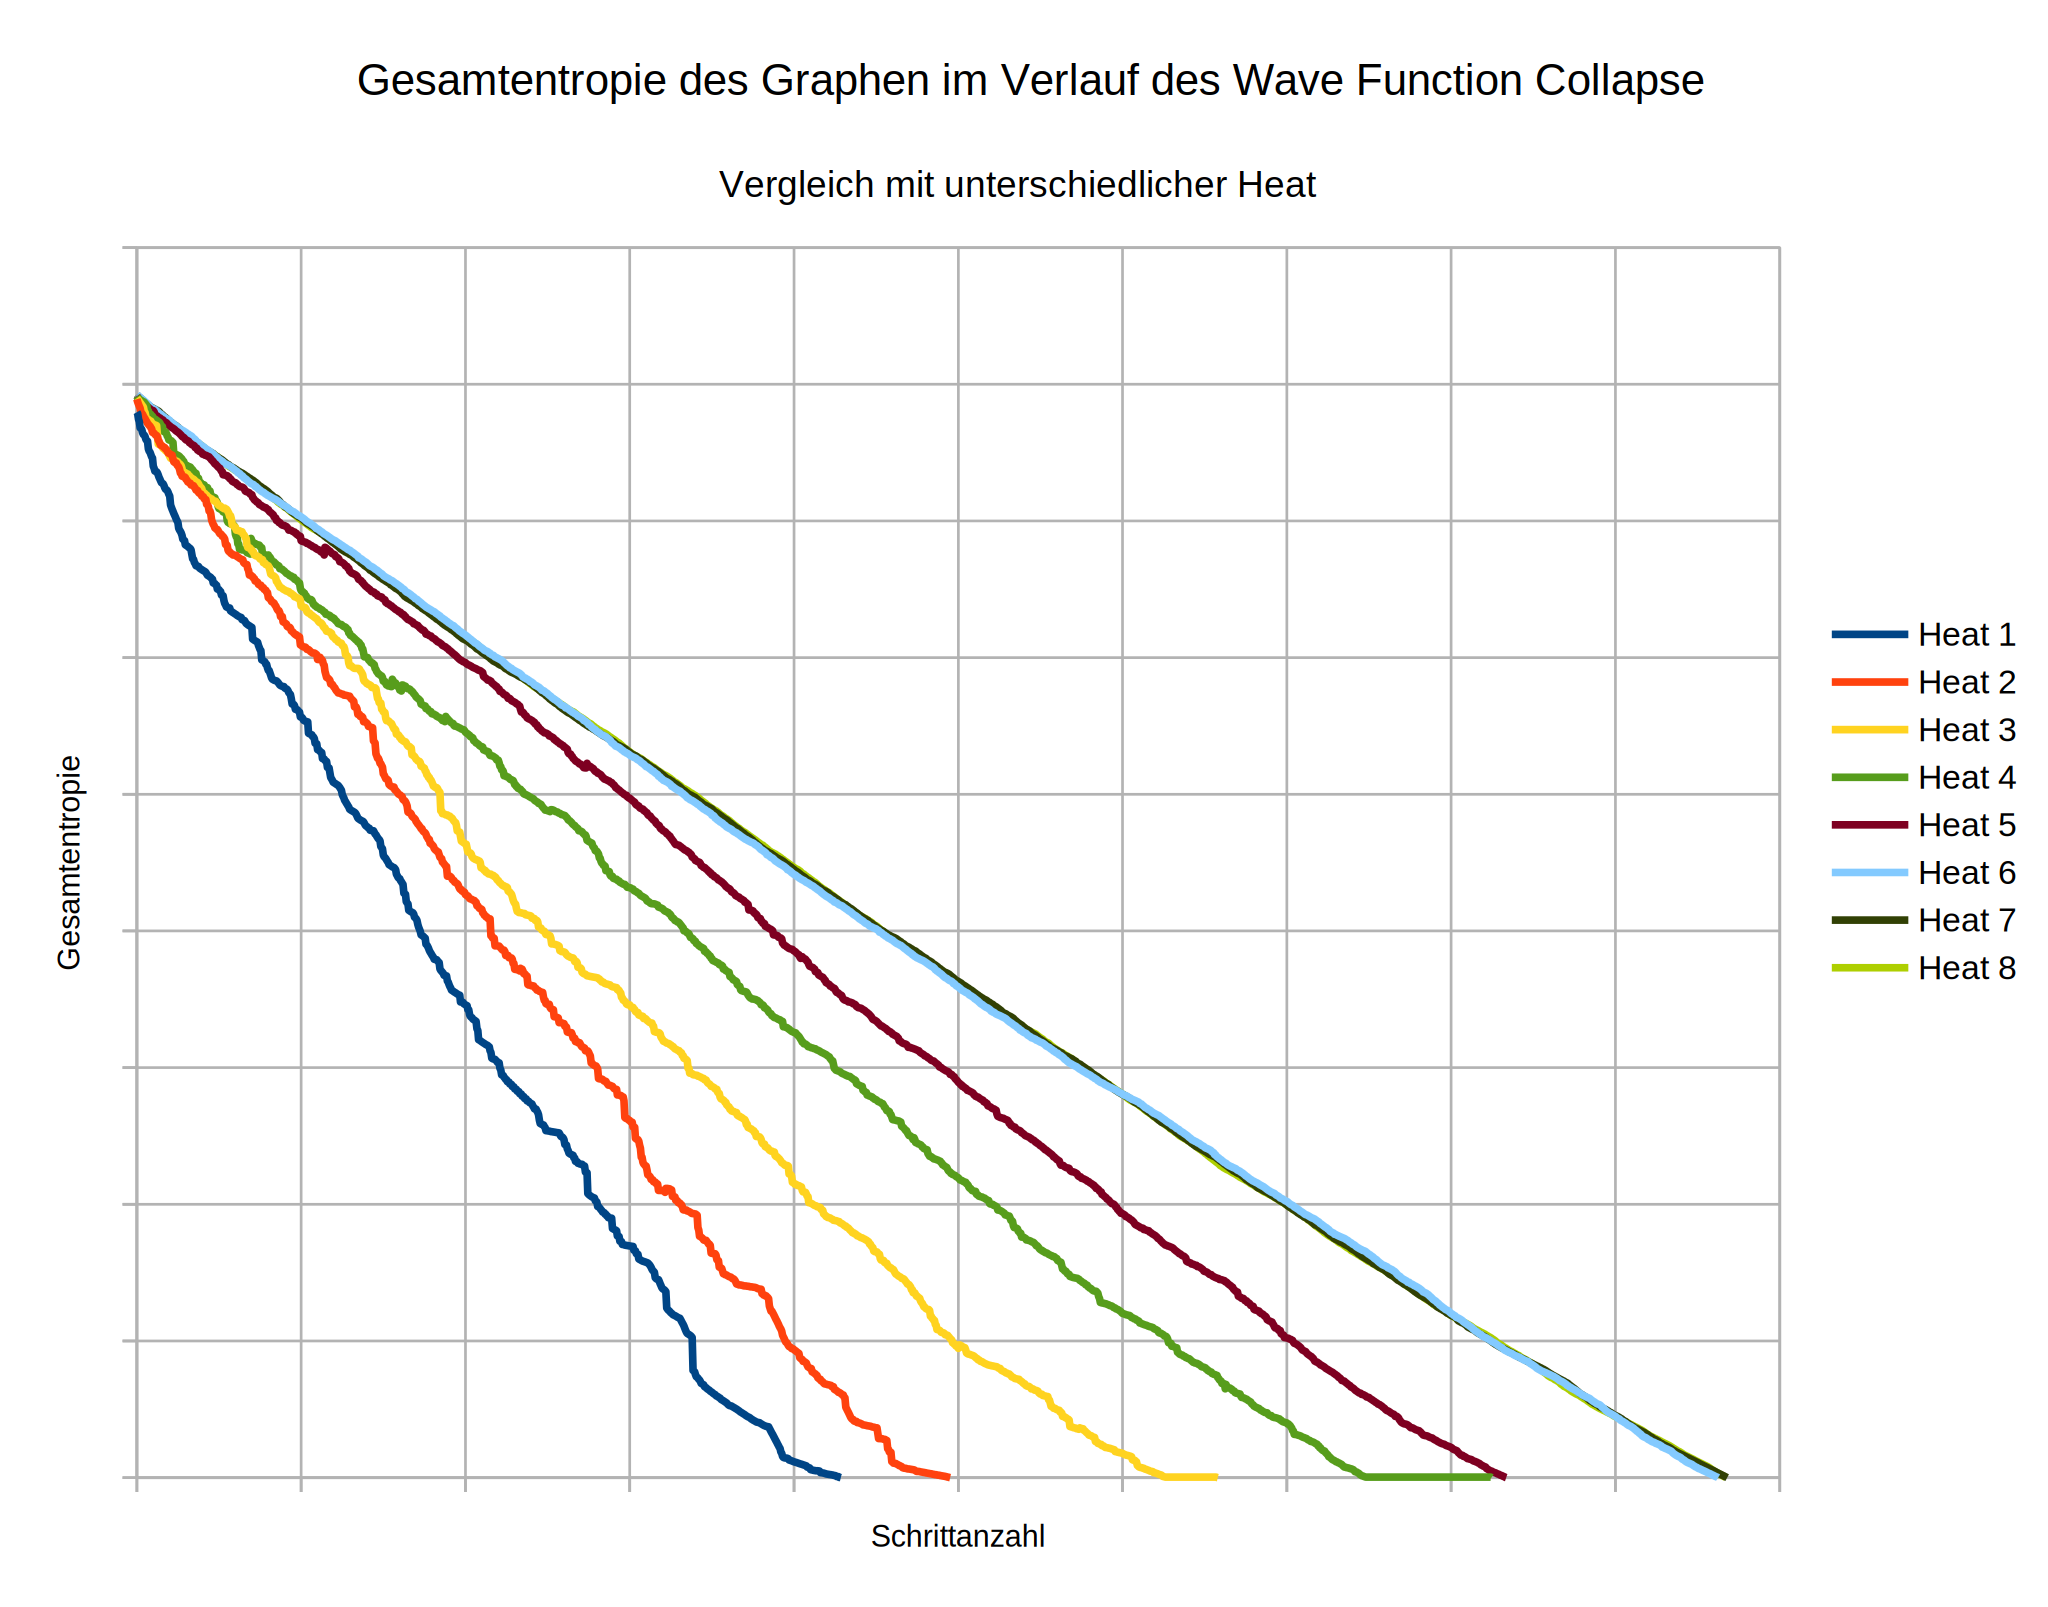
\includegraphics[width=\linewidth]{data/townscaper_grid/1.png} \caption{} \end{subfigure}
    \begin{subfigure}{0.18\textwidth} \includegraphics[width=\linewidth]{data/townscaper_grid/2.png} \caption{} \end{subfigure}
    \begin{subfigure}{0.18\textwidth} \includegraphics[width=\linewidth]{data/townscaper_grid/3.png} \caption{} \end{subfigure}
    \begin{subfigure}{0.18\textwidth} \includegraphics[width=\linewidth]{data/townscaper_grid/4.png} \caption{} \end{subfigure}
    \begin{subfigure}{0.18\textwidth} \includegraphics[width=\linewidth]{data/townscaper_grid/5.png} \caption{} \end{subfigure}
    
    \caption{
        Generierung eines Teils des Gitters für Townscaper \cite{stalberg_grid}. (a) Punkte werden generiert. (b) Triangulierung. (c) Kanten werden gelöscht, so dass Vierecke entstehen. (d) die Vierecke werden geviertelt. (e) Position der Knoten wird aufgelockert, so dass die Winkel zwischen Kanten gleichmäßiger sind.
    }
    \label{fig:townscaper_grid}
\end{figure}
    
    
    \section{Wave Function Collapse}
        \textit{Wave Function Collapse} \cite{gumin} ist eine Weiterentwicklung des Model Sythesis Algorithmus \ref{alg:wfc_gumin}. Abbildung \ref{fig:wfc_overview} zeigt einige Beispiele und daraus generierte Bilder. Der Name ist eine Anspielung auf die Quantenphysik. So könnte man Quantenpartikel in Superposition mit den Zellen des Gitters vergleichen. Die Zellen haben auch mehrere mögliche finale Zustände bis sie observiert werden und in einen festen Zustand kollabiert. Mathematisch besteht aber keine Beziehung. Auch werden andere Begriffe wie z.B. Knoten zu Zelle umbenannt und das Gitter als Wave bezeichnet. Die Kernidee der Generierung mittels einem Beispiel bleibt und wird um drei Aspekte erweitert:
        
        \begin{enumerate}
        \item Bauteile können automatisch aus einem Beispiel extrahiert werden.
        \item Im Algorithmus werden die Zellen beginnend mit der niedrigsten Entropie abgearbeitet. 
        \item Spiegelungen und Reflexionen von Bauteilen werden automatisch erzeugt und verwendet.
        \end{enumerate}
        
        \begin{figure}[ht]
    \centering
    \begin{minipage}{\linewidth}
        \rule{\linewidth}{0.4pt}
        
        \begin{enumerate}
        \item Read the input bitmap and count NxN patterns.
        \subitem (optional) Augment pattern data with rotations and reflections.
        \item Create an array with the dimensions of the output (called ''wave'' in the source). Each element of this array represents a state of an NxN region in the output. A state of an NxN region is a superposition of NxN patterns of the input with boolean coefficients (so a state of a pixel in the output is a superposition of input colors with real coefficients). False coefficient means that the corresponding pattern is forbidden, true coefficient means that the corresponding pattern is not yet forbidden.
        \item Initialize the wave in the completely unobserved state, i.e. with all the boolean coefficients being true.
        \item Repeat the following steps: \begin{enumerate}
            \item Observation: \begin{enumerate}
                \item Find a wave element with the minimal nonzero entropy. If there is no such elements (if all elements have zero or undefined entropy) then break the cycle (4) and go to step (5).
                \item Collapse this element into a definite state according to its coefficients and the distribution of NxN patterns in the input.
            \end{enumerate}
            \item Propagation: propagate information gained on the previous observation step.
        \end{enumerate}
        \item By now all the wave elements are either in a completely observed state (all the coefficients except one being zero) or in the contradictory state (all the coefficients being zero). In the first case return the output. In the second case finish the work without returning anything.
        \end{enumerate}
        
        \rule{\linewidth}{0.4pt}
    \end{minipage}
    
    \caption{Wave Function Collapse Algorithmus nach Gumin \cite{gumin}}
    
    \label{fig:wfc_gumin}
\end{figure}
        \begin{figure}[H]
    \centering
    \begin{subfigure}{0.18\textwidth} 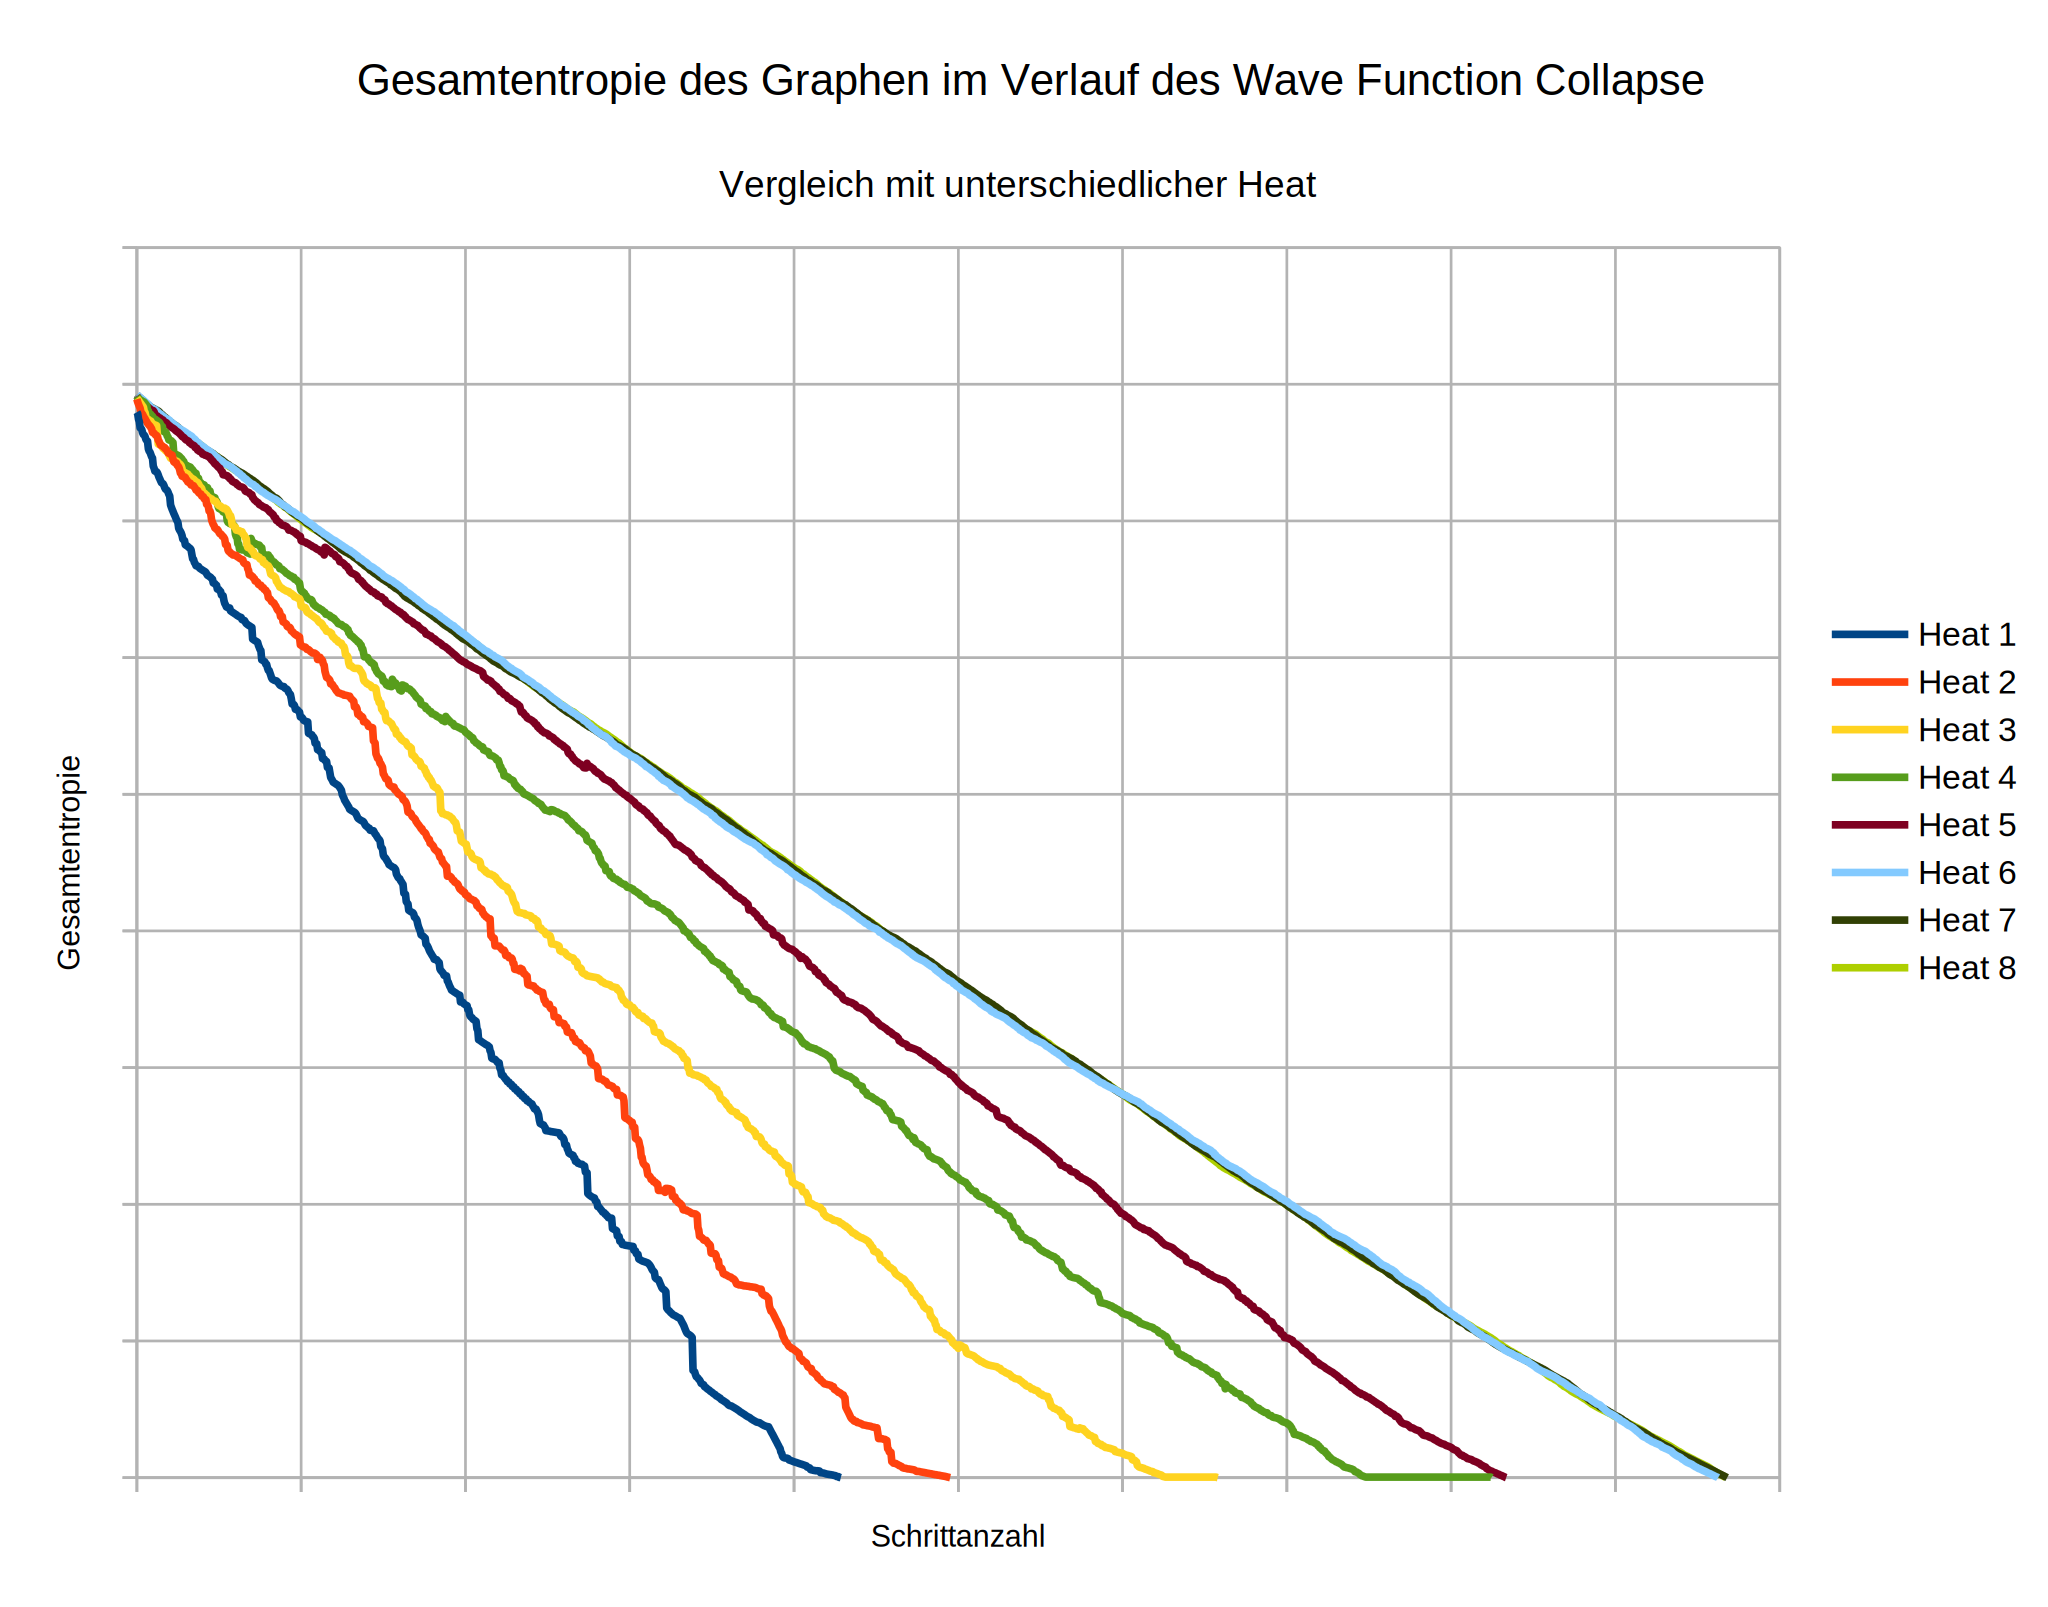
\includegraphics[width=\linewidth]{data/townscaper_grid/1.png} \caption{} \end{subfigure}
    \begin{subfigure}{0.18\textwidth} \includegraphics[width=\linewidth]{data/townscaper_grid/2.png} \caption{} \end{subfigure}
    \begin{subfigure}{0.18\textwidth} \includegraphics[width=\linewidth]{data/townscaper_grid/3.png} \caption{} \end{subfigure}
    \begin{subfigure}{0.18\textwidth} \includegraphics[width=\linewidth]{data/townscaper_grid/4.png} \caption{} \end{subfigure}
    \begin{subfigure}{0.18\textwidth} \includegraphics[width=\linewidth]{data/townscaper_grid/5.png} \caption{} \end{subfigure}
    
    \caption{
        Generierung eines Teils des Gitters für Townscaper \cite{stalberg_grid}. (a) Punkte werden generiert. (b) Triangulierung. (c) Kanten werden gelöscht, so dass Vierecke entstehen. (d) die Vierecke werden geviertelt. (e) Position der Knoten wird aufgelockert, so dass die Winkel zwischen Kanten gleichmäßiger sind.
    }
    \label{fig:townscaper_grid}
\end{figure}
        \pagebreak
        
        \subsection{Entropie}
            Bei Model Synthesis werden Zellen einfach nach ihrer Reihenfolge im Gitter abgearbeitet. Der Vorteil ist, dass keine Suche der nächsten Zelle nötig ist, aber es hat zum Nachteil, dass die Ausgabe sichtbare Artefakte enthällt (siehe Abbildung \ref{fig:directional_bias}). Man kann erkennen, ob zuerst die Reihen oder erst die Spalten abgearbeitet wurden. Wäre bekannt welche Zelle den meisten Fortschritt zur Lösung und die geringste Chance auf einen Widerspruch birgt, könnte stets diese Zelle zuerst betrachtet werden. 
            
            \begin{figure}[H]
    \centering
    \begin{subfigure}{0.18\textwidth} 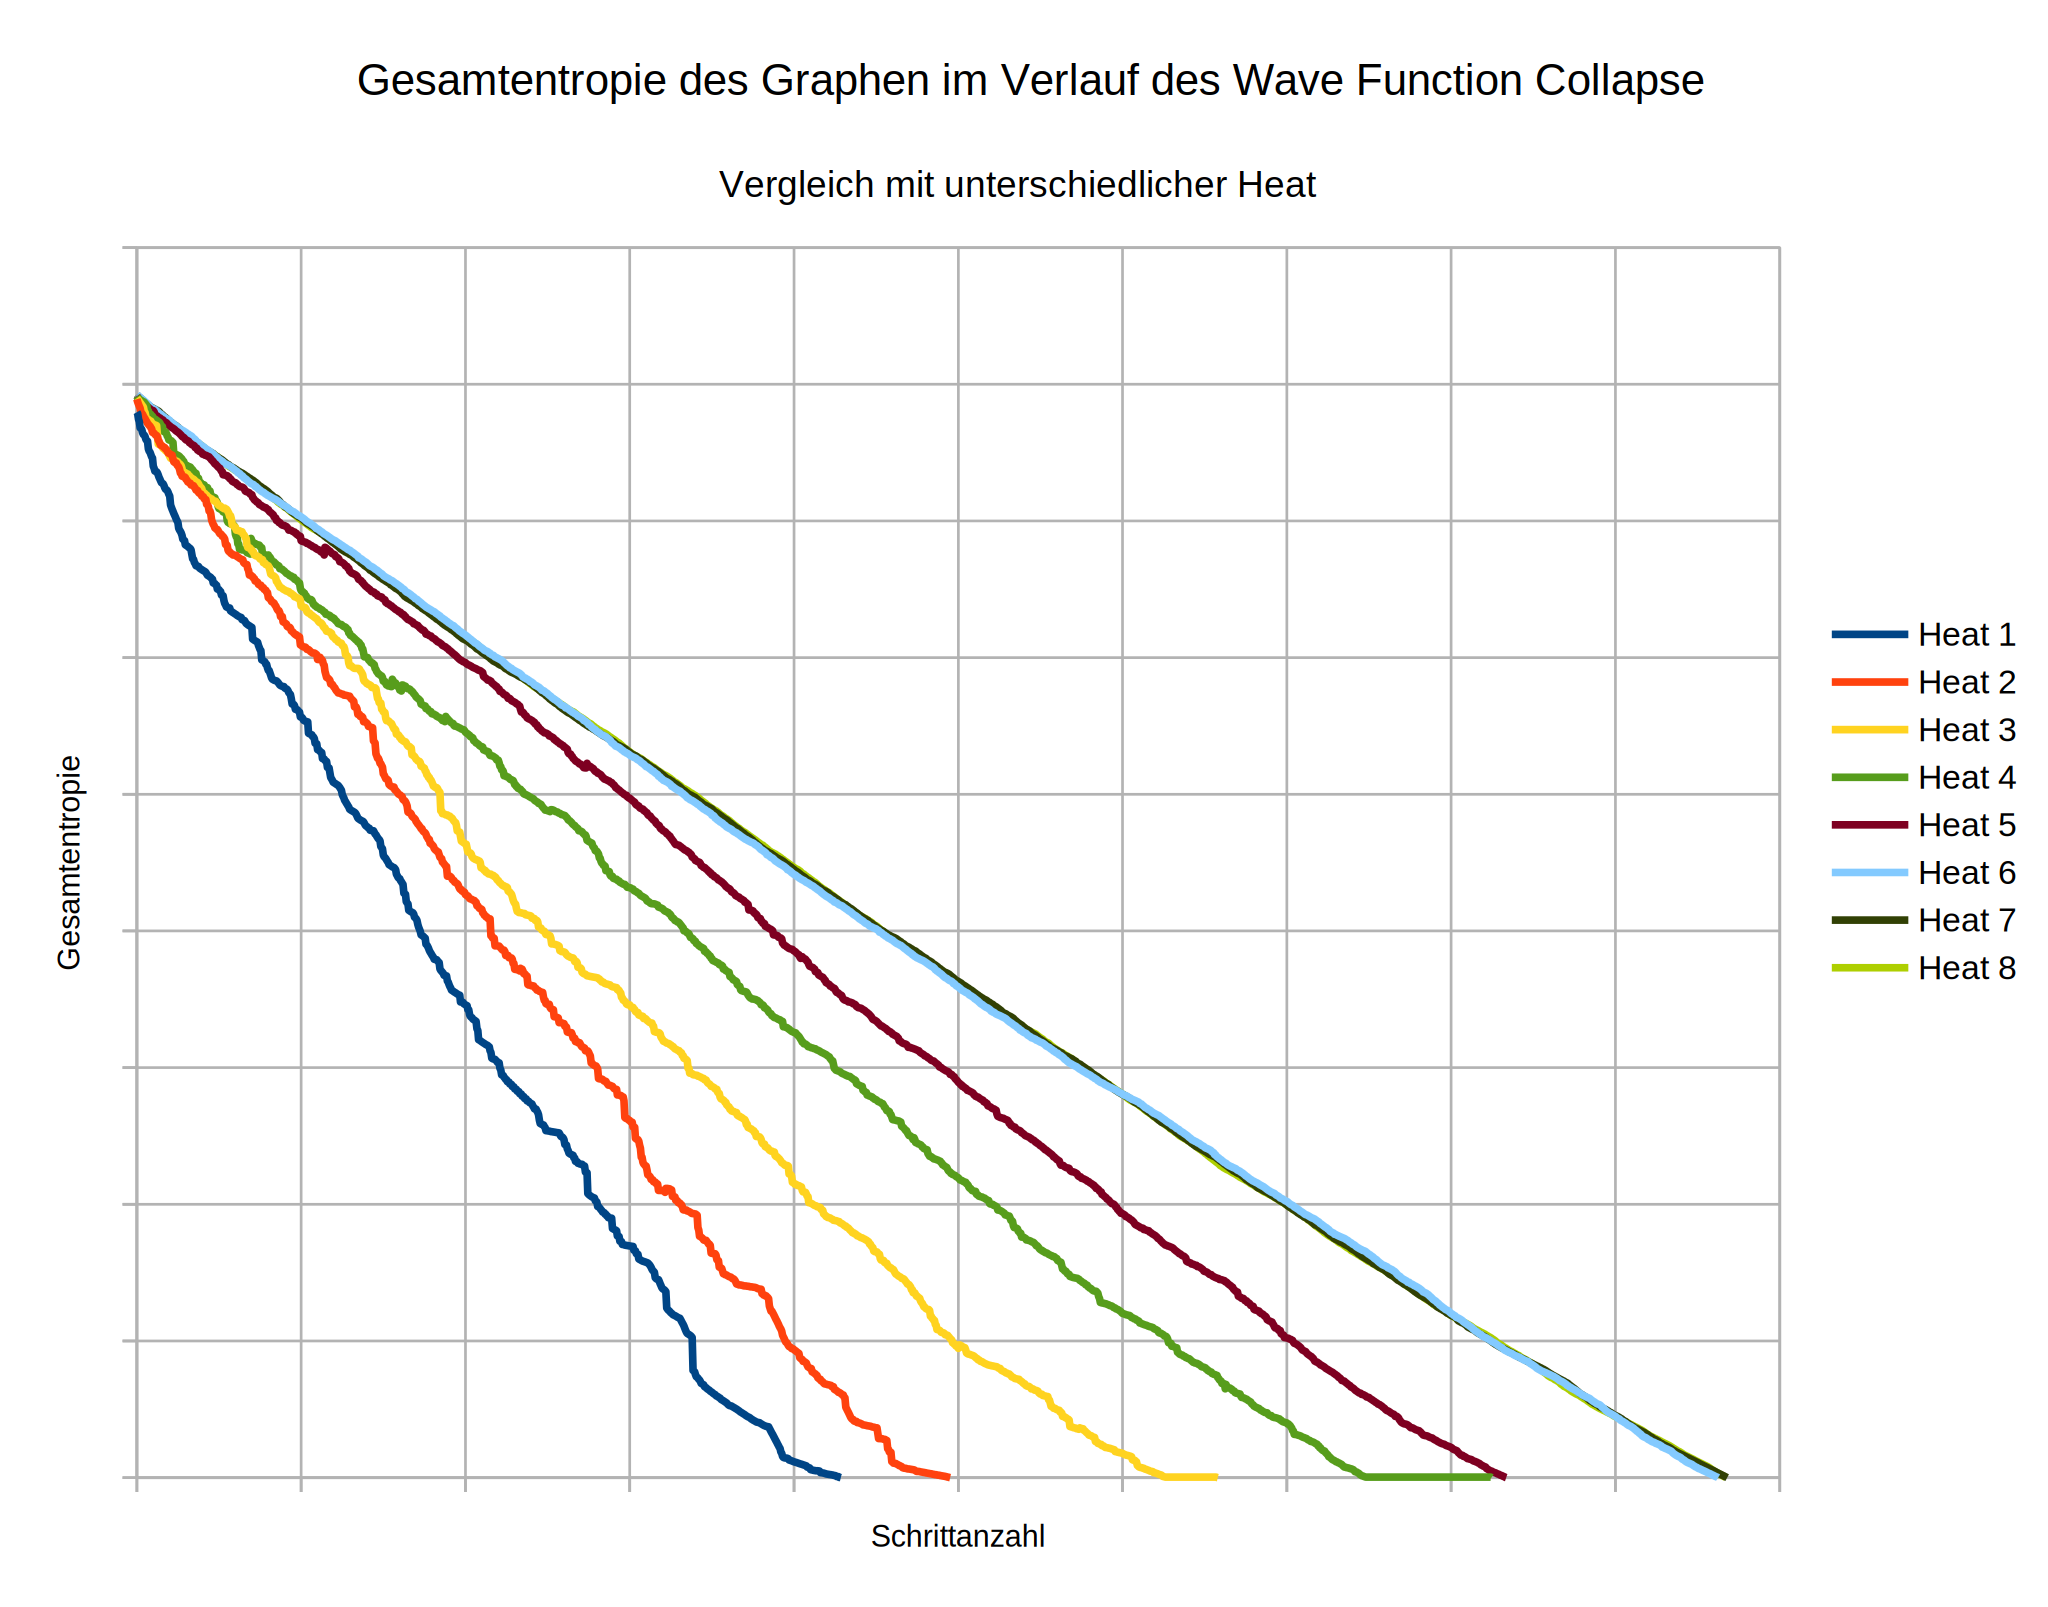
\includegraphics[width=\linewidth]{data/townscaper_grid/1.png} \caption{} \end{subfigure}
    \begin{subfigure}{0.18\textwidth} \includegraphics[width=\linewidth]{data/townscaper_grid/2.png} \caption{} \end{subfigure}
    \begin{subfigure}{0.18\textwidth} \includegraphics[width=\linewidth]{data/townscaper_grid/3.png} \caption{} \end{subfigure}
    \begin{subfigure}{0.18\textwidth} \includegraphics[width=\linewidth]{data/townscaper_grid/4.png} \caption{} \end{subfigure}
    \begin{subfigure}{0.18\textwidth} \includegraphics[width=\linewidth]{data/townscaper_grid/5.png} \caption{} \end{subfigure}
    
    \caption{
        Generierung eines Teils des Gitters für Townscaper \cite{stalberg_grid}. (a) Punkte werden generiert. (b) Triangulierung. (c) Kanten werden gelöscht, so dass Vierecke entstehen. (d) die Vierecke werden geviertelt. (e) Position der Knoten wird aufgelockert, so dass die Winkel zwischen Kanten gleichmäßiger sind.
    }
    \label{fig:townscaper_grid}
\end{figure}
            \pagebreak
            
            Merrel zeigt im Anhang seines Papers \cite{merrel}, dass die Entscheidung, ob eine Ausgabe vervollständigt werden kann, ein NP-vollständiges Problem ist. Einfacher ist es eine Heuristik zu definieren. Hierfür wird die Shannon-Entropie \cite{shannon} als Maß eingeführt. Sie beschreibt das Maß an Ungewissheit in einem System, hier die Ungewissheit über den finalen Zustand einer Zelle. Sie wird mit der Formel \ref{eq:entropy} berechnet, wobei $\mathcal{X}$ die Menge der möglichen Zustände einer Zelle ist und $p(x)$ die Wahrscheinlichkeit das $x$ gewählt wird ist.
            
            Ist eine Zelle observiert, hat sie nur noch einen Zustand und die Entropie ist 0, während eine Zelle mit vielen Möglichkeiten eine hohe Entropie hat. Die Entropie gibt auch Information darüber wie sehr eine Zelle durch ihre Umgebung beschränkt wird, weil Zellen mit vielen Beschränkungen nur noch wenige mögliche Zustände haben.  
                       
            %     % \caption{
%     %     Formel für die Shannon-Entropie. 
%     %     $\mathcal{X}$ ist die Menge der Möglichen Zustände einer Zelle.
%     %     $p(x)$ ist die Wahrscheinlichkeit das $x$ gewählt wird.
%     % }

\begin{equation}
    \label{eq:entropy}
    \mathrm{entropy}(\mathcal{X}) = -\sum_{x \in \mathcal{X}} p(x),\log p(x)
\end{equation}
        
        
        \subsection{Symmetrie}
            Ziel des Model Synthesis Algorithmus ist es, eine große Anzahl lokal ähnlicher Ausgaben zu generieren \cite{merrel}. Ähnlichkeit wird erreicht, wenn jede kleine Region der Ausgabe zu Regionen des Beispiels passt (siehe Abbildung \ref{fig:wfc_resemblance}). Die wahrgenommene Ähnlichkeit wird verbessert, wenn das Verhältnis der Häufigkeiten von Regionen der Verteilung im Beispiel gleicht. Im Wave Function Collapse wird dieses Kriterium erweitert. Die Regionen können nun auch Drehungen und Spiegelungen der Regionen im Beispiel sein \cite{gumin}.
            
            \begin{figure}[H]
    \centering
    \begin{subfigure}{0.18\textwidth} 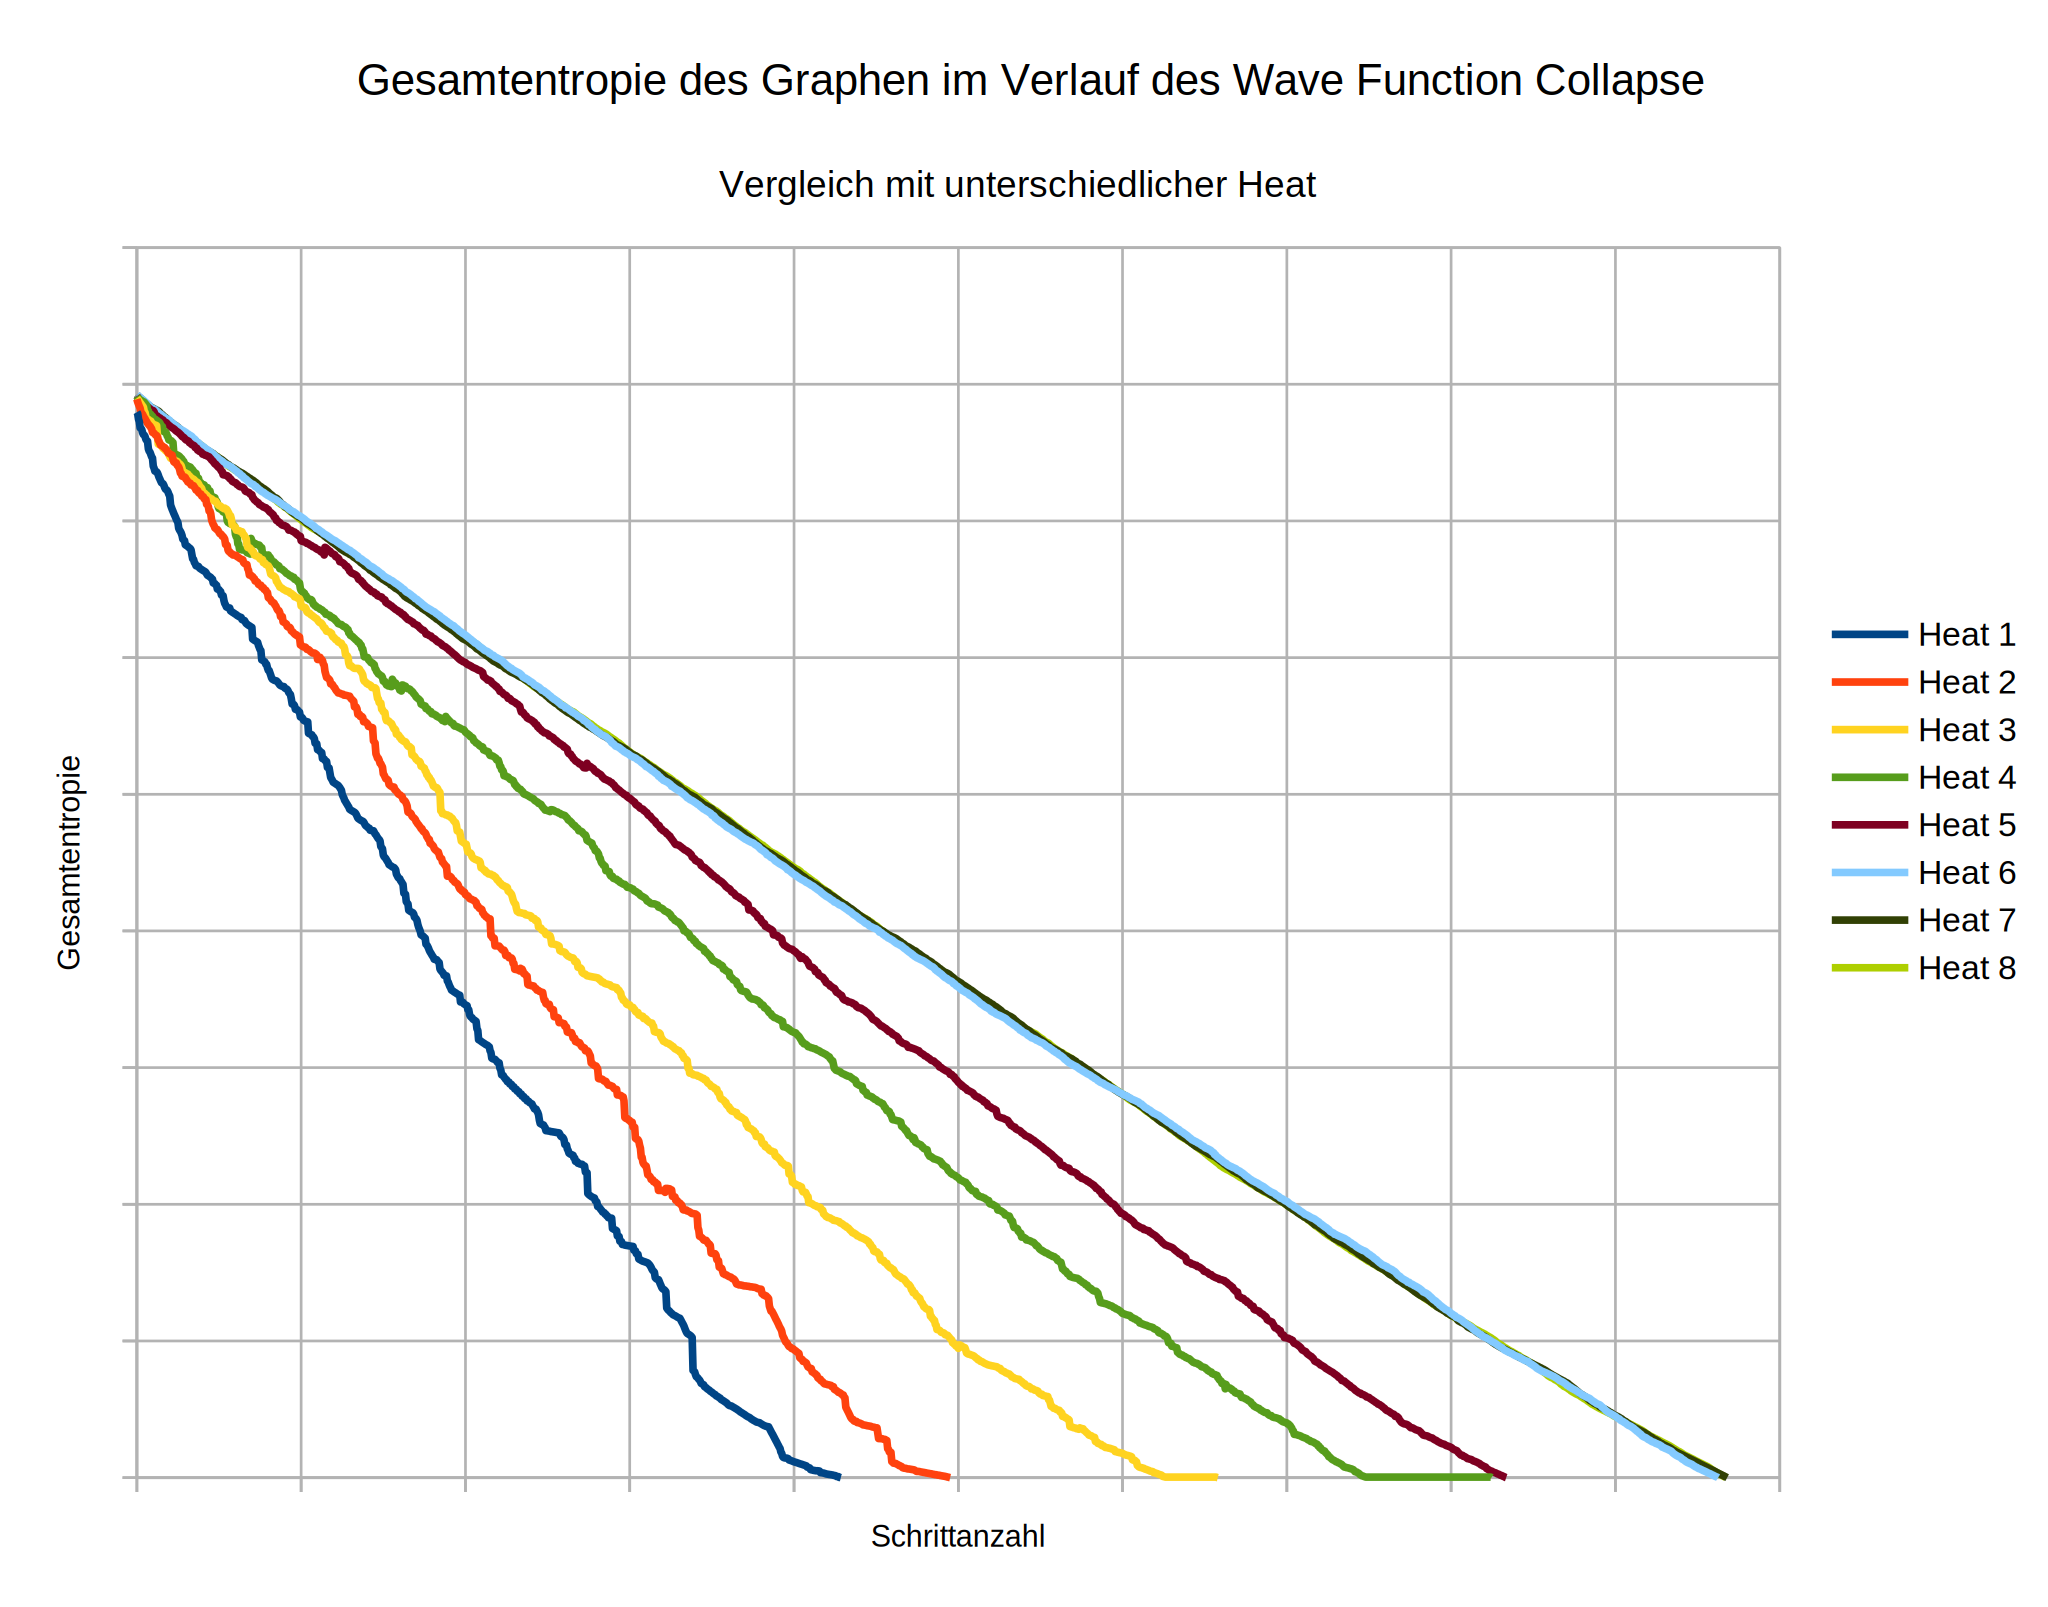
\includegraphics[width=\linewidth]{data/townscaper_grid/1.png} \caption{} \end{subfigure}
    \begin{subfigure}{0.18\textwidth} \includegraphics[width=\linewidth]{data/townscaper_grid/2.png} \caption{} \end{subfigure}
    \begin{subfigure}{0.18\textwidth} \includegraphics[width=\linewidth]{data/townscaper_grid/3.png} \caption{} \end{subfigure}
    \begin{subfigure}{0.18\textwidth} \includegraphics[width=\linewidth]{data/townscaper_grid/4.png} \caption{} \end{subfigure}
    \begin{subfigure}{0.18\textwidth} \includegraphics[width=\linewidth]{data/townscaper_grid/5.png} \caption{} \end{subfigure}
    
    \caption{
        Generierung eines Teils des Gitters für Townscaper \cite{stalberg_grid}. (a) Punkte werden generiert. (b) Triangulierung. (c) Kanten werden gelöscht, so dass Vierecke entstehen. (d) die Vierecke werden geviertelt. (e) Position der Knoten wird aufgelockert, so dass die Winkel zwischen Kanten gleichmäßiger sind.
    }
    \label{fig:townscaper_grid}
\end{figure}
            
            Desweiteren wird auch eine Annotation für manuell erstellten Bauteile definiert, mit der ein Nutzer einem Bauteil eine Symmetriegruppe zuweisen kann \cite{gumin}. Eine Symmetriegruppe gibt an, wie man ein Bauteil drehen und spiegeln kann. Beim Einlesen generiert der Algorithmus basiert auf dieser Symmetriegruppe weitere, entsprechend gedreht oder gespiegelte, Bauteil die im weiteren Prozess verwendet werden. Da sich diese Arbeit nicht mit Beispielen aus Bauteilen befässt sondern primär diese automatisch extrahiert, bleibt dieser Aspekt ungenutzt.
        
        
        \subsection{Extraktion}
            Zuvor musste der Nutzer das gewünschte Beispielmodell oder Beispielbild manuell in einzelne gleichgroße Bauteile zerlegen, aus denen der Algorithmus dann neue Modelle und Bilder generiert. Wave Function Collapse nutzt einen Algorithmus \ref{alg:wfc_extraction} zur Generierung dieser Bauteile \cite{gumin}. Die größe der Bauteile ist dabei freiwählbar, aber sie sollte so gewählt sein, das sie zum genutzen Beispiel passt, damit die im Beispiel existierenden Muster erhalten bleiben.  Sind die Bauteile zu klein gewählt, gehen Strukturen des Beispiels verloren. Während zu große Bauteile auch unerwünschte Strukturen im Beispiel enthalten, was im extremen Fall dazu führt, dass nur noch exakte Kopien des Beispiels ohne Variation in der Ausgabe vorkommen. Für Bilder wird in dieser Arbeit stets die Moore-Nachbarschaft jedes Pixels, also die direkt angrenzenden Pixel sowie die entlang der Diagonalen, als Bauteil verwendet. Dies wird auch als das Umfeld des Pixels beschrieben.
            
            \begin{algorithm}
    \caption{Regelextraktion}
    \label{alg:wfc_extraction}
    
    \begin{enumerate}
    \item Für jeden Pixel des Beispielbilds:
        \begin{enumerate}
        \item Überschreitet das Umfeld des Pixels den Rand des Bild?
        \subitem Ist Wrapping erlaubt?
        \subsubitem Dann: Nimm die Pixel vom gegenüberliegenden Rand
        \subsubitem Sonst: Überspringe diesen Pixel
        \item Lese das Umfeld aus
        \item Gibt es bereits einen Zustand mit diesem Umfeld?
        \subitem Dann: Erhöhe dessen Frequenz um eins
        \subitem Sonst: Erstelle einen neuen Zustand mit diesem Umfeld
        \end{enumerate}
    
    \item Für jedes Paar Zustände und jede Himmelsrichtung:
        \begin{enumerate}
        \item Prüfe ob die Zustände in dieser Richtung überlappen
        \item Speichere diese Regel in der Lookuptabelle ab
        \end{enumerate}
    \end{enumerate}
        
\end{algorithm}
            
            In Abbildung \ref{fig:extract_wrapping} ist der Ablauf dargestellt. Aus dem Beispiel werden die Umfelder ausgelesen. Die kann mit oder ohne \textit{Wrapping} passieren, wobei Wrapping bedeutet, dass wenn z.B. der rechte Rand überschritten wird, es zurück zum linken Rand und von da aus weiter geht. Dies kann separat für die vertikalen Ränder und die horizontalen Ränder erlaubt oder verboten werden. Die Zustände ergeben sich aus den einzigartigen Umfelder. Die Frequenz eines Umfelds gibt an wie oft es im Beispiel vorkommt. Sind mehrere Umfelder gleich, so hat der entsprechende Zustand einen höhere Frequenz. Aus der Gesamtanzahl an Zuständen und deren Frequenzen lässt sich die Wahrscheinlichkeit jedes Zustands gewählt zu werden berechen. Im Algorithmus wird dies beachtet, damit die globale Verteilung von Zuständen in der Ausgabe der Verteilung im Beispiel ähnelt. Danach wird geprüft, welche der gefundenen Zustände überlappen. Es werden die Himmelrichtungen N, S, W und O geprüft und für später in einer Lookuptabelle gespeichert.
            
            \begin{figure}[H]
    \centering
    \begin{subfigure}{0.18\textwidth} 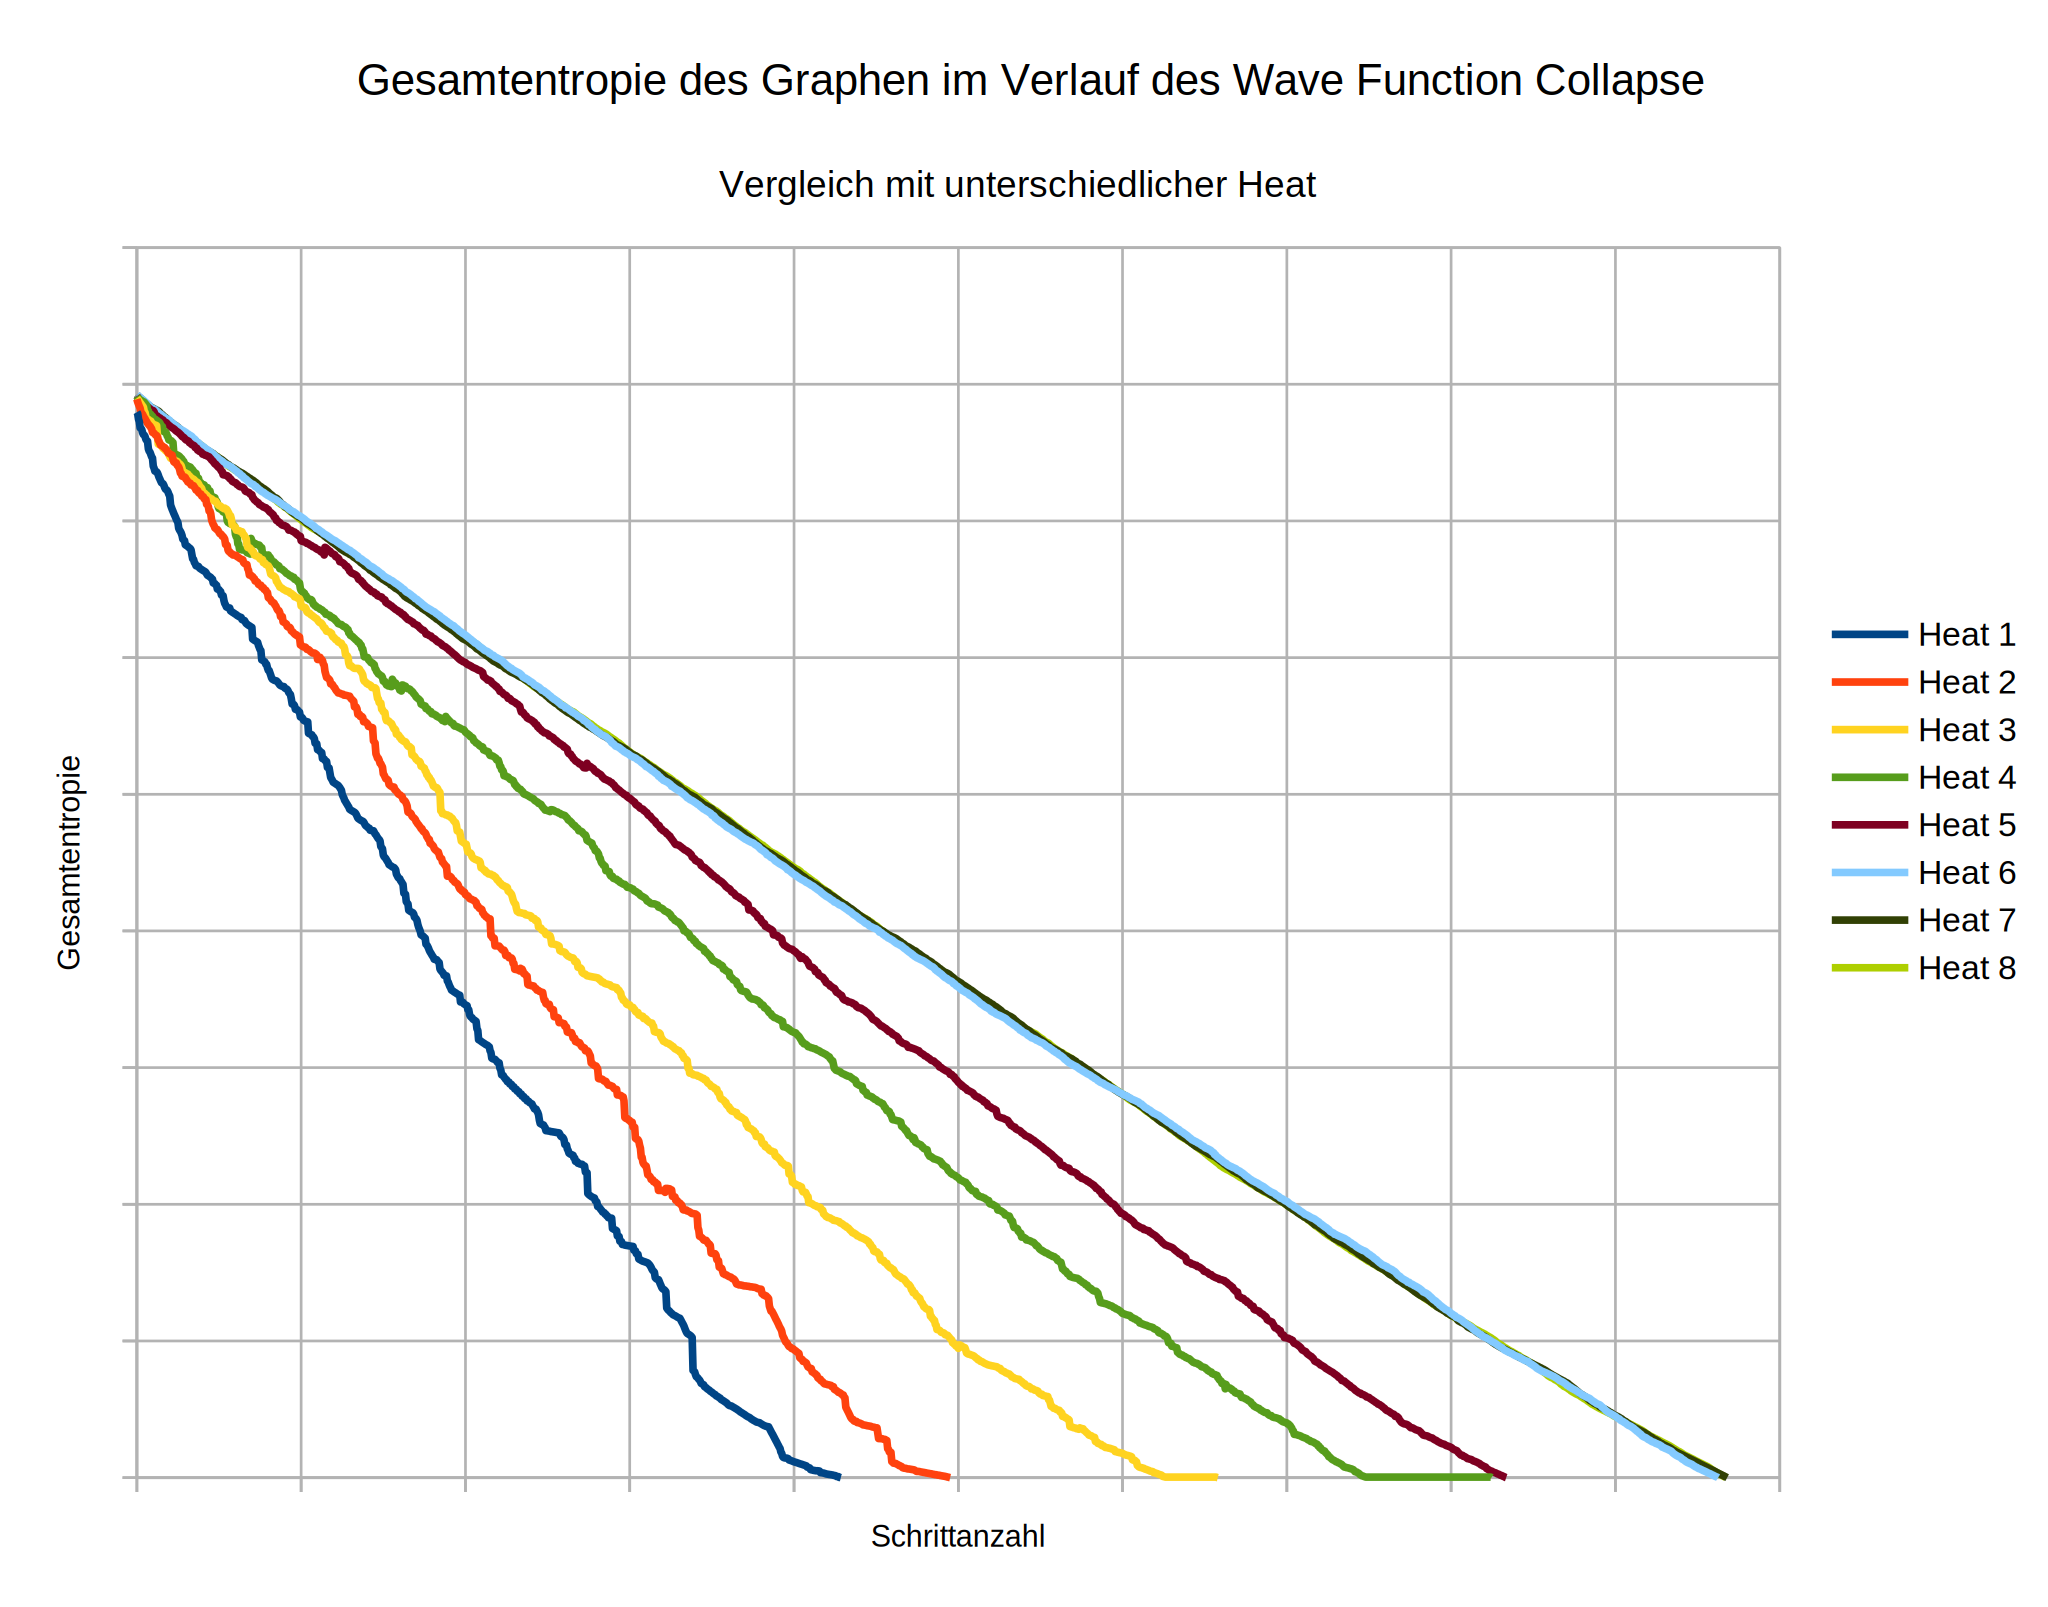
\includegraphics[width=\linewidth]{data/townscaper_grid/1.png} \caption{} \end{subfigure}
    \begin{subfigure}{0.18\textwidth} \includegraphics[width=\linewidth]{data/townscaper_grid/2.png} \caption{} \end{subfigure}
    \begin{subfigure}{0.18\textwidth} \includegraphics[width=\linewidth]{data/townscaper_grid/3.png} \caption{} \end{subfigure}
    \begin{subfigure}{0.18\textwidth} \includegraphics[width=\linewidth]{data/townscaper_grid/4.png} \caption{} \end{subfigure}
    \begin{subfigure}{0.18\textwidth} \includegraphics[width=\linewidth]{data/townscaper_grid/5.png} \caption{} \end{subfigure}
    
    \caption{
        Generierung eines Teils des Gitters für Townscaper \cite{stalberg_grid}. (a) Punkte werden generiert. (b) Triangulierung. (c) Kanten werden gelöscht, so dass Vierecke entstehen. (d) die Vierecke werden geviertelt. (e) Position der Knoten wird aufgelockert, so dass die Winkel zwischen Kanten gleichmäßiger sind.
    }
    \label{fig:townscaper_grid}
\end{figure}

    \section{Visualisierung}
        Die Ausgabe der Wave Function Collapse muss nicht direkt bildlich verwendet werden. Welche Bedeutung die Zellen und deren Zustände haben, ist dem Algorithmus egal. Dieser garantiert nur lokale Ähnlichkeit zum Beispiel. Im erfolgreiche Spiel \textit{Townscaper} \cite{stalberg_townscaper} von Oskar Stålberg wird Wave Function Collapse verwendet. In Abbildung \ref{fig:townscaper} sind einige Screenshots aus dem Spiel zu sehen.
        
        
        Hier kann die Spielerin aus Gebäuden eine Stadt bauen. Sie wählt dabei aber nicht die konkreten Gebäude aus, sondern legt nur fest, welche Art/Farbe an jeweiliger Stelle platziert werden soll. Das Spiel nutzt Wave Function Collapse, um die dementsprechend am besten passenden Gebäudeteile zu finden. Danach wird das gewählte Modell an den Knotenpunkt angepasst und mit Details wie Fensters oder Bänken ausgeschmückt.
        
        
        Damit die Stadt nicht geradlinig verläuft, wird sie auf einer spezielle Art von Gitter gebaut. Abbildung \ref{fig:townscaper_grid} zeigt, wie die Teile, aus denen das Gitter besteht, generiert werden. Es ist zu erkennen, dass es auf einer Quadrilierung, aufbaut. Eine Quadrilierung ist ein Graph, dessen Kanten Vierecke bilden. Die sechseckigen Regionen werden im Spiel zusammengesetzt und an den Knoten kann die Spielerin Gebäude bauen. Die meisten Knotenpunkte haben vier Kanten, aber es gibt auch einzelne mit drei oder fünf Kanten. Im Spiel existieren für diese Arten von Knoten jeweils unterschiedliche Modelle von Gebäuden. Es müssen keine weiteren Modelle, für willkürlich viele Kanten an einem Knoten, erstellt werden, da dieser Prozess nur diese drei Arten von Knoten generiert. Es handelt sich also nicht um eine allgemeine Lösung, da die Beispielmodelle speziell für das genutzt Gitter erstellt wurden und nicht für anderen Art von Graphen funktionieren würden.
        
        \begin{figure}[H]
    \centering
    \begin{subfigure}{0.18\textwidth} 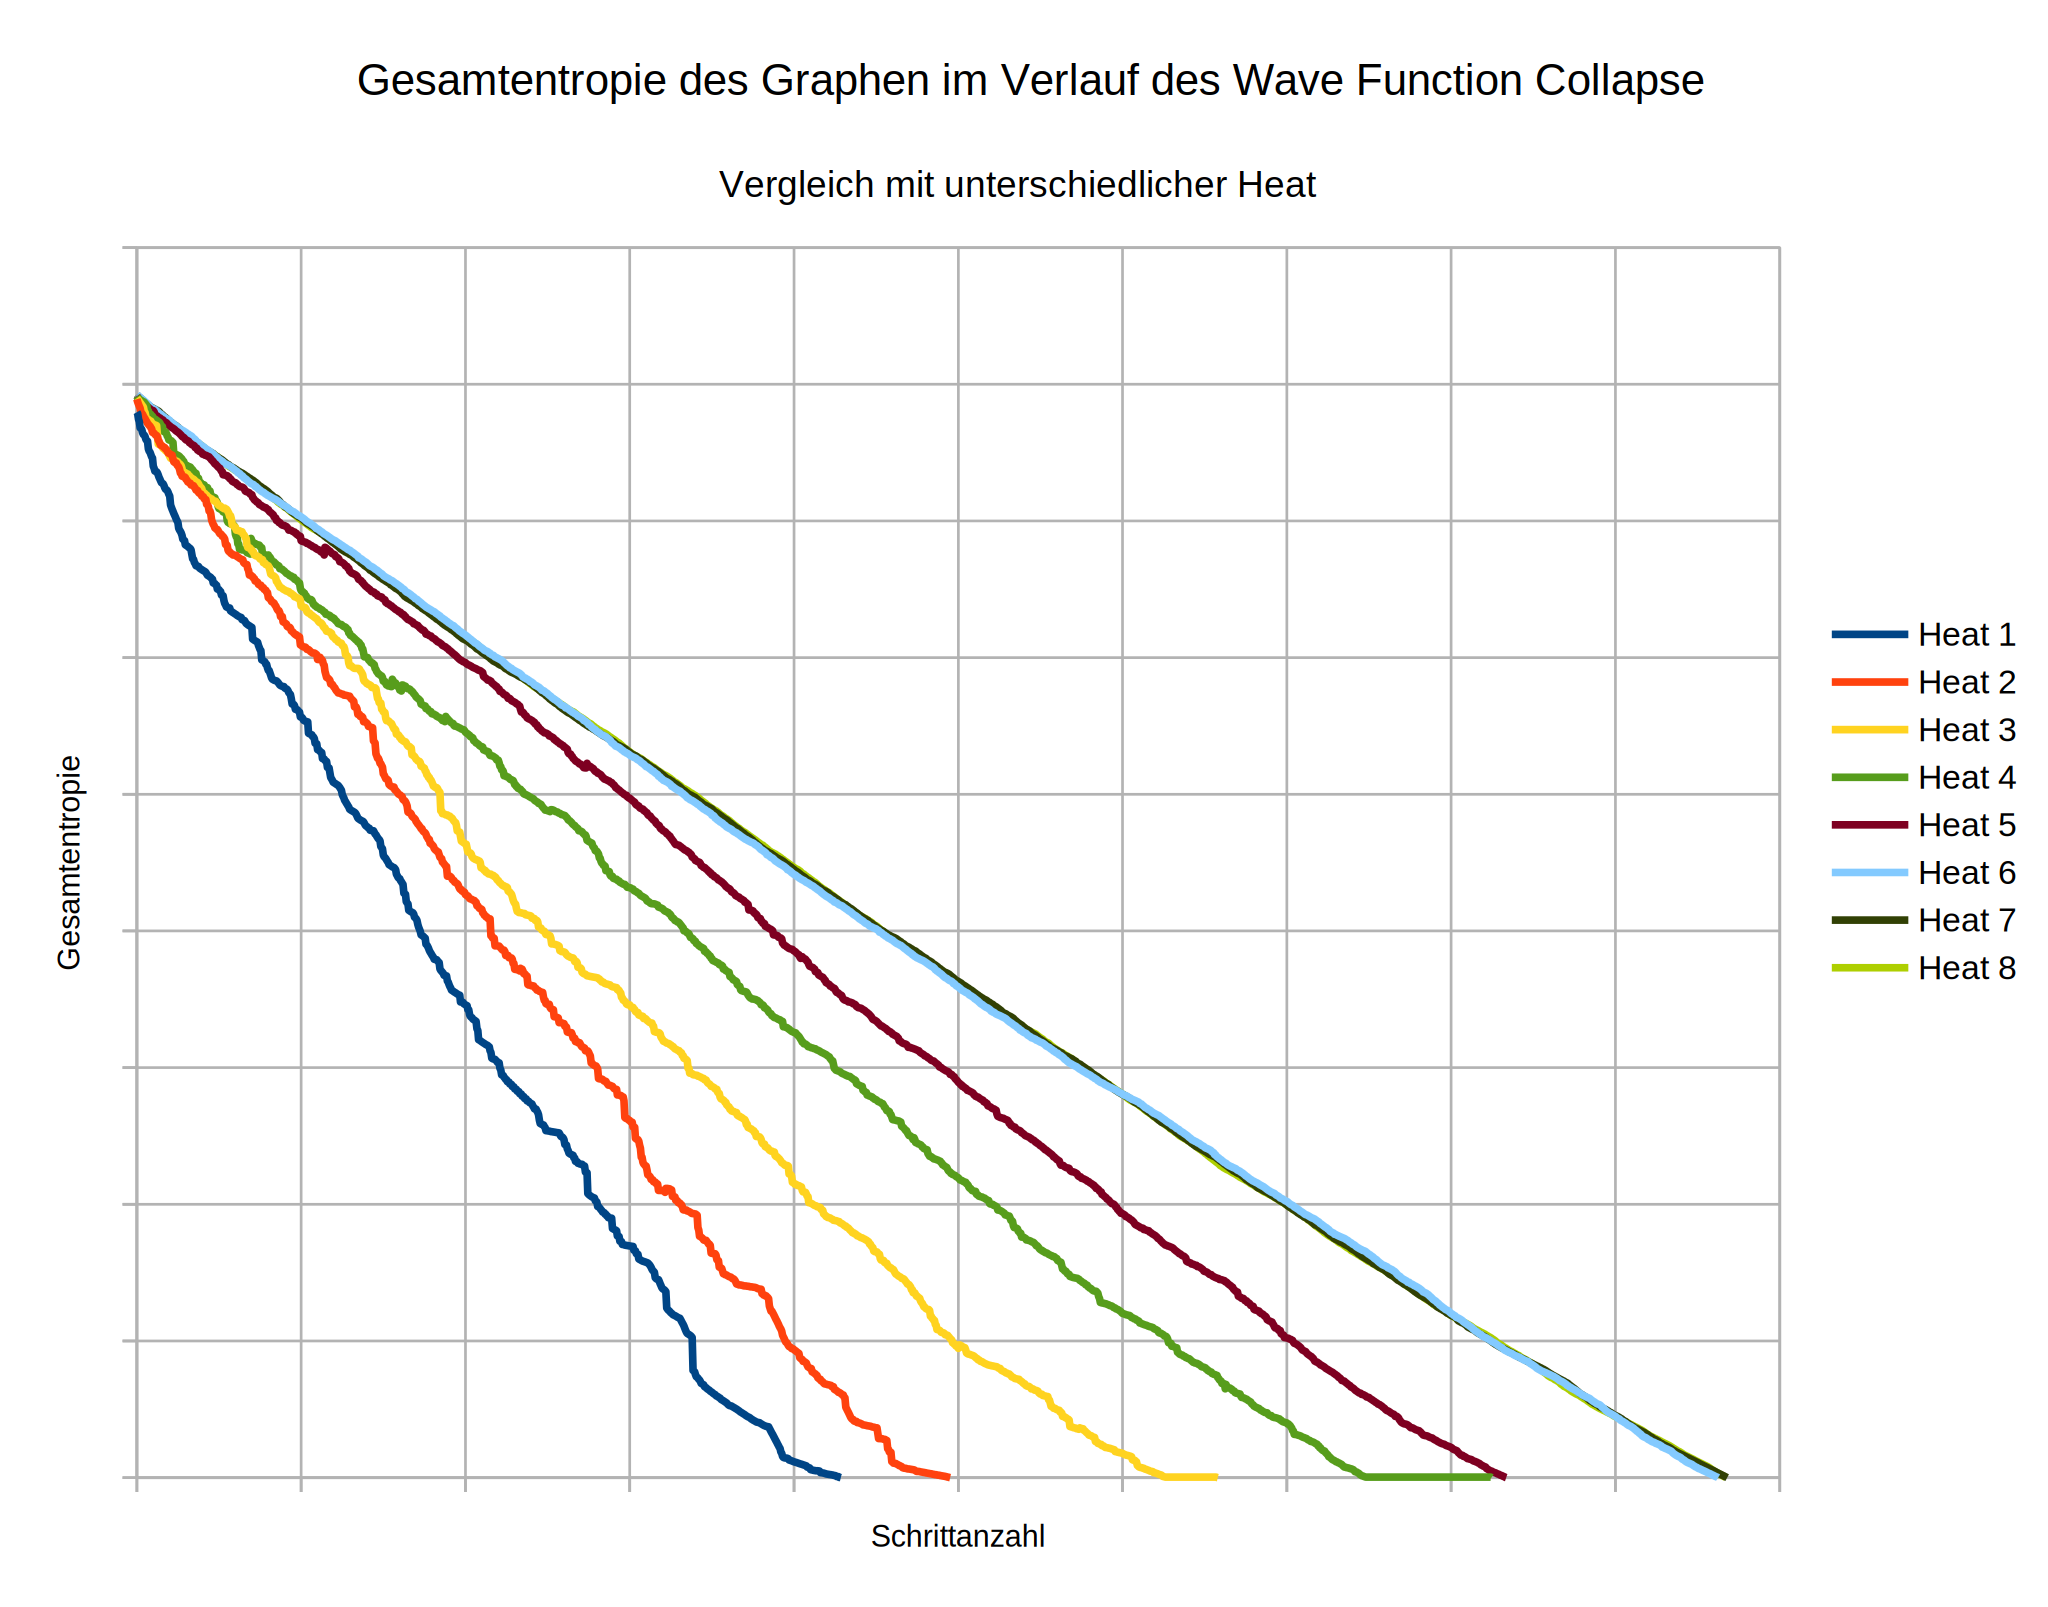
\includegraphics[width=\linewidth]{data/townscaper_grid/1.png} \caption{} \end{subfigure}
    \begin{subfigure}{0.18\textwidth} \includegraphics[width=\linewidth]{data/townscaper_grid/2.png} \caption{} \end{subfigure}
    \begin{subfigure}{0.18\textwidth} \includegraphics[width=\linewidth]{data/townscaper_grid/3.png} \caption{} \end{subfigure}
    \begin{subfigure}{0.18\textwidth} \includegraphics[width=\linewidth]{data/townscaper_grid/4.png} \caption{} \end{subfigure}
    \begin{subfigure}{0.18\textwidth} \includegraphics[width=\linewidth]{data/townscaper_grid/5.png} \caption{} \end{subfigure}
    
    \caption{
        Generierung eines Teils des Gitters für Townscaper \cite{stalberg_grid}. (a) Punkte werden generiert. (b) Triangulierung. (c) Kanten werden gelöscht, so dass Vierecke entstehen. (d) die Vierecke werden geviertelt. (e) Position der Knoten wird aufgelockert, so dass die Winkel zwischen Kanten gleichmäßiger sind.
    }
    \label{fig:townscaper_grid}
\end{figure}
        \begin{figure}[H]
    \centering
    \begin{subfigure}{0.18\textwidth} \includegraphics[width=\linewidth]{data/townscaper_grid/1.png} \caption{} \end{subfigure}
    \begin{subfigure}{0.18\textwidth} \includegraphics[width=\linewidth]{data/townscaper_grid/2.png} \caption{} \end{subfigure}
    \begin{subfigure}{0.18\textwidth} \includegraphics[width=\linewidth]{data/townscaper_grid/3.png} \caption{} \end{subfigure}
    \begin{subfigure}{0.18\textwidth} \includegraphics[width=\linewidth]{data/townscaper_grid/4.png} \caption{} \end{subfigure}
    \begin{subfigure}{0.18\textwidth} \includegraphics[width=\linewidth]{data/townscaper_grid/5.png} \caption{} \end{subfigure}
    
    \caption{
        Generierung eines Teils des Gitters für Townscaper \cite{stalberg_grid}. (a) Punkte werden generiert. (b) Triangulierung. (c) Kanten werden gelöscht, so dass Vierecke entstehen. (d) die Vierecke werden geviertelt. (e) Position der Knoten wird aufgelockert, so dass die Winkel zwischen Kanten gleichmäßiger sind.
    }
    \label{fig:townscaper_grid}
\end{figure}
